\documentclass[11pt, a4paper]{article}
\usepackage{multicol}
\usepackage{tikz}
\usepackage{tikz,fullpage}
\usetikzlibrary{arrows,%
	petri,%
	topaths}%
\usepackage{tkz-berge}
\usepackage{amsmath}
\usepackage{amsfonts}
\usepackage{amssymb}

\usepackage{textcomp}
\usepackage{logicproof}
\usepackage{float}
\usepackage[hidelinks]{hyperref}
\usepackage[T1]{fontenc}
\usepackage[]{algorithm2e}
\usepackage{parskip}
\usepackage[toc,page]{appendix}
\usepackage{graphicx}
\usepackage{subcaption}
\usepackage{multirow}
\usepackage[lmargin=0.3in,rmargin=0.3in,tmargin=0.3in,bmargin=0.6in]{geometry}

\graphicspath{  {../Saved_Figs/} {../Dataset/} }
%opening
\title{\vspace{-1.25cm}Machine Learning Coursework - OULAD Analysis}
\author{mbtj48}
\date{}

\begin{document}

\maketitle
\vspace{-0.4cm}
\begin{multicols}{2}
\section{Data Gathering and Analysis}

Machine learning and data gathering are paramount for modern, cutting edge technologies. Thus we have been tasked to develop two machine learning models to predict final grades from the OULAD.

\begin{figure}[H]
	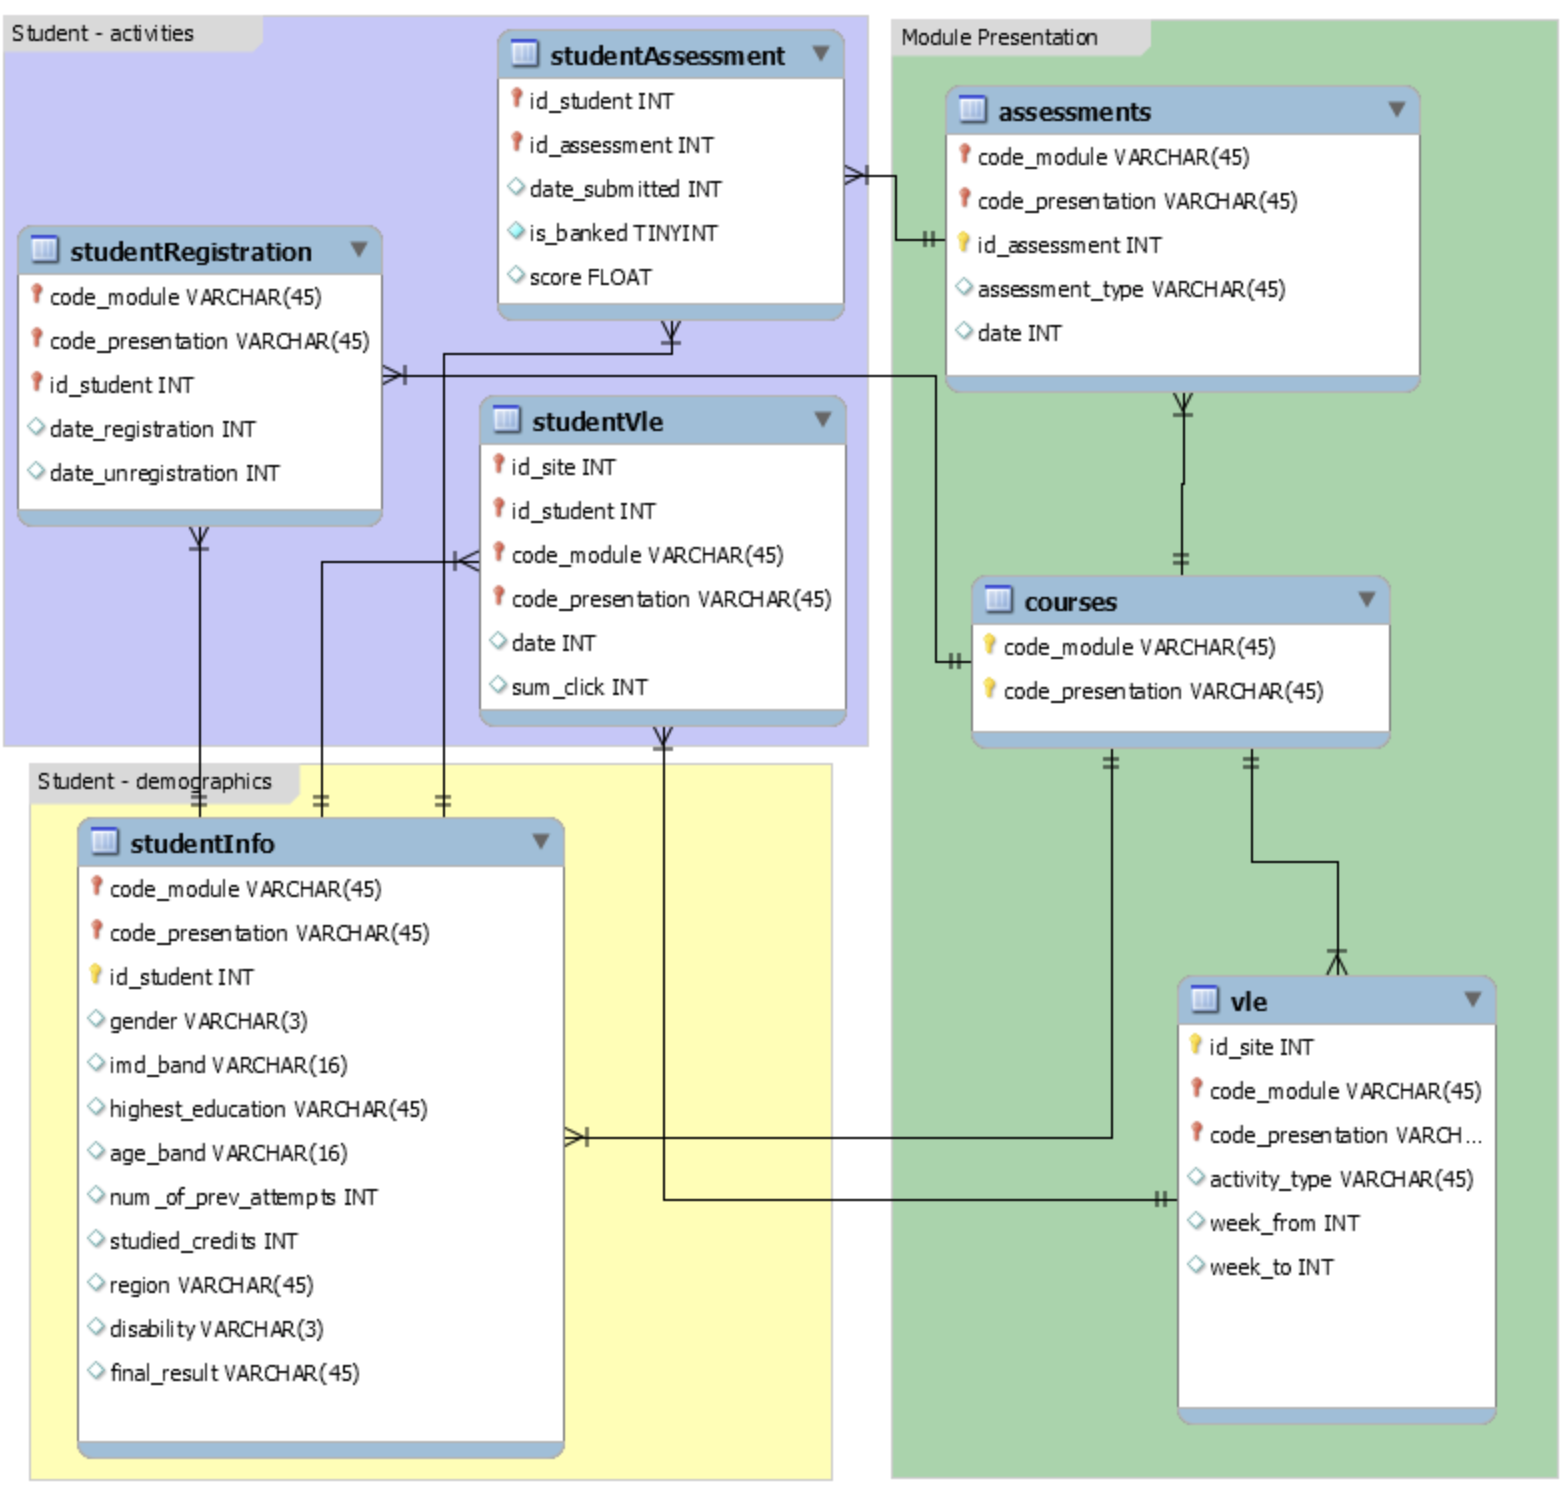
\includegraphics[width=\linewidth]{dataset.png} 
	\caption{Dataset Schema}
	\label{fig:schema}
\end{figure}
\vspace{-0.4cm}
Firstly, I noticed useful features such as the score in the studentAssessment table, and sum-click in the studentVle table.
Therefore I started by grouping the sum-click and score features, finding the net clicks within the portal for a given student through the year and their average mark. 
I expected these features to show a positive correlation because higher scores and grades generally correlate with high effort [tab \ref{table:Correlations}].
Then, I plotted the data and noticed that a logistic regression model should perform highly. 
I added more data to my model; intending to use as much data as possible to aid the model in finding patterns: ie calculating how many days early they submitted coursework and their summative and formative (weight $= 0$) marks. 
As the student would be more prepared and committed, I expected a positive correlation from this data.

My interpretation of the data evolved as, I included a wide range of the available data, thus I started to interpret the data differently: including the mean, median, mean absolute deviation, standard deviation and variance for different data in the schema.
I then produced a correlation heatmap [fig \ref{fig:heatmap}], plus the sorted numerical correlations [tab \ref{table:Correlations}].


\begin{table}[H]
	\centering
	\begin{tabular}{|l|l|}
		\hline
		\textbf{Feature}                    & \textbf{Correlation} \\ \hline
		daysEarlystdScore            & $-0.259014$ \\ \hline
		studied-credits             & $-0.176016$ \\ \hline
		region-Wales                & $0.008382$  \\ \hline
		age-band                    & $0.068551$  \\ \hline
		score                        & $0.317339$  \\ \hline
		sum-click                   & $0.376107$  \\ \hline
		totalCoursework              & $0.427175$  \\ \hline
		summativeAgainstCredits      & $0.490646$  \\ \hline
		\end{tabular}
		\caption{Correlations}
		\label{table:Correlations}
\end{table}


Surprisingly, age-band shows a weak correlation; in theory, you would expect a mild negative correlation. However, this could be due to limited data (3 unique ranges - [fig \ref{fig:LinAge}]). To improve this correlation, I would need more spread out ranges or use integers instead of the ranges.

After data gathering, I preprocessed the data with an imputer and scaler. The imputer changes all NA values to the median of that feature. 
While the scaler, normalises features to be within $0-1$, this prevents feature domination with large ranges and makes the features unit dependent.
Further, I exchanged region, code module and code presentation to columned data by one-hot encoding those categories.
\vspace{-0.4cm}
\section{Model Selection}

The following phase involved selecting models. Here, I split the data into train and test sets with a 75/25 split; then tested a variety of models and compared how they performed in cross-validation on the training data. 
Generally, there was a wide performance range, with classifiers generally doing better than regressors. See table \ref{table:modelSelection} for further information. I decided to pick one regressor and one classifier to explore: Logistic Regression and Random Forest Classifier.
\vspace{-0.4cm}
\section{Model A - Logistic Regression}

Moving on to hyperparameter tuning: For this model, I decided to use a grid search to validate the best combination within the domain. I explored a logarithmic range of the C parameter; until after testing, I reached an optimal range of 950-1100. It also checked tolerance values around the default, ending with 0.0015.
The other set of combinations check the same values of C and adjust the solver and penalty used. Finally, I removed the second set of combinations as it did not help to increase performance.
\vspace{-0.4cm}
\section{Model B - Random Forest Classifier}

Initially, I used Random Search to tune the classifier. This generates parameters to cross-validate the model.
I decided to check the number of estimators, the maximum depth, the minimum number of samples and the minimum number of samples required to split an internal node.
I moved on to use Bayesian optimisation to optimise this search problem. This uses the previous iterations to strategically select the next best parameters from the search space to minimise the loss function. I defined the loss as $ 3 - \overline{acc} - \overline{acc_{bal}} - \overline{f1_{weighted}}$; this, therefore, seeks to reduce the primary metrics for a classification problem.
Next, I removed the unimportant attributes from the forest's feature importances [fig \ref{fig:importances}] and tuned the model again. I noticed the number of estimators showed little correlation for the model improving the loss function [fig \ref{fig:estimators}] and this second tune slightly improved the model [figs \ref{fig:Acc1} $\to$ \ref{fig:Acc2}].
\vspace{-0.4cm}
\section{Conclusion}

\begin{table}[H]
	\centering
	% \renewcommand{\arraystretch}{1.2}
	\begin{tabular}{|p{3.4cm}|c|c|c|c|}
	  \hline
	  \textbf{Model} & \multicolumn{2}{c|}{\textbf{Logistic}} & \multicolumn{2}{c|}{\textbf{Random Forest}}\\
	  \cline{2-5}\hline
	  \textbf{Classes}& \textbf{2} & \textbf{4} & \textbf{2} & \textbf{4}\\
	  \hline
	  Explained Var 									& 0.697 & 0.664 & 0.823 & 0.729  \\ \hline
	  RMSE 												& 0.275 & 0.585 & 0.213 & 0.523  \\ \hline
	  MAE 												& 0.076 & 0.300 & 0.045 & 0.263  \\ \hline
	  r2 Score 											& 0.697 & 0.662 & 0.819 & 0.729  \\ \hline
	  f1 Score (weighted)\newline (Recall and Precision) & 0.924 & 0.706 & 0.955 & 0.739  \\ \hline
	  Accuracy 											& 0.924 & 0.721 & 0.955 & 0.742  \\ \hline
	\end{tabular}
	\caption{Metrics of Final Models}
	\label{table:metrics}
  \end{table}

  The logistic regression model finished with an accuracy of 0.721\%, while the random forest classifier finished with 0.742\%.
  Although notably, the weighted average of the f1 score for both models are lower; which is likely a better metric to measure, as it reduces metric skew on imbalanced data. Furthermore, upon analysing the classification report, classes with low balance have lower performance due to the data imbalance.
  The confusion matrices [tables \ref{table:RF4Confusion},\ref{table:RF2Confusion},\ref{table:Log4Confusion},\ref{table:Log2Confusion}] showed that "close" classes such as withdrawn and fail and pass and distinction are easily mistaken.
  Finally, note the two-class metrics (these merge withdrawn and fail \& pass and distinction, as these are subclasses of the primary labels) which are generally high performing. The random forest 2-class model would be good to implement to determine whether a given student is likely to fail, due to the high accuracy and f1 score [\ref{table:metrics}].

% \newpage
\section*{Appendix}
\centering
\begin{figure}[H]
	\vspace{-0.4cm}
	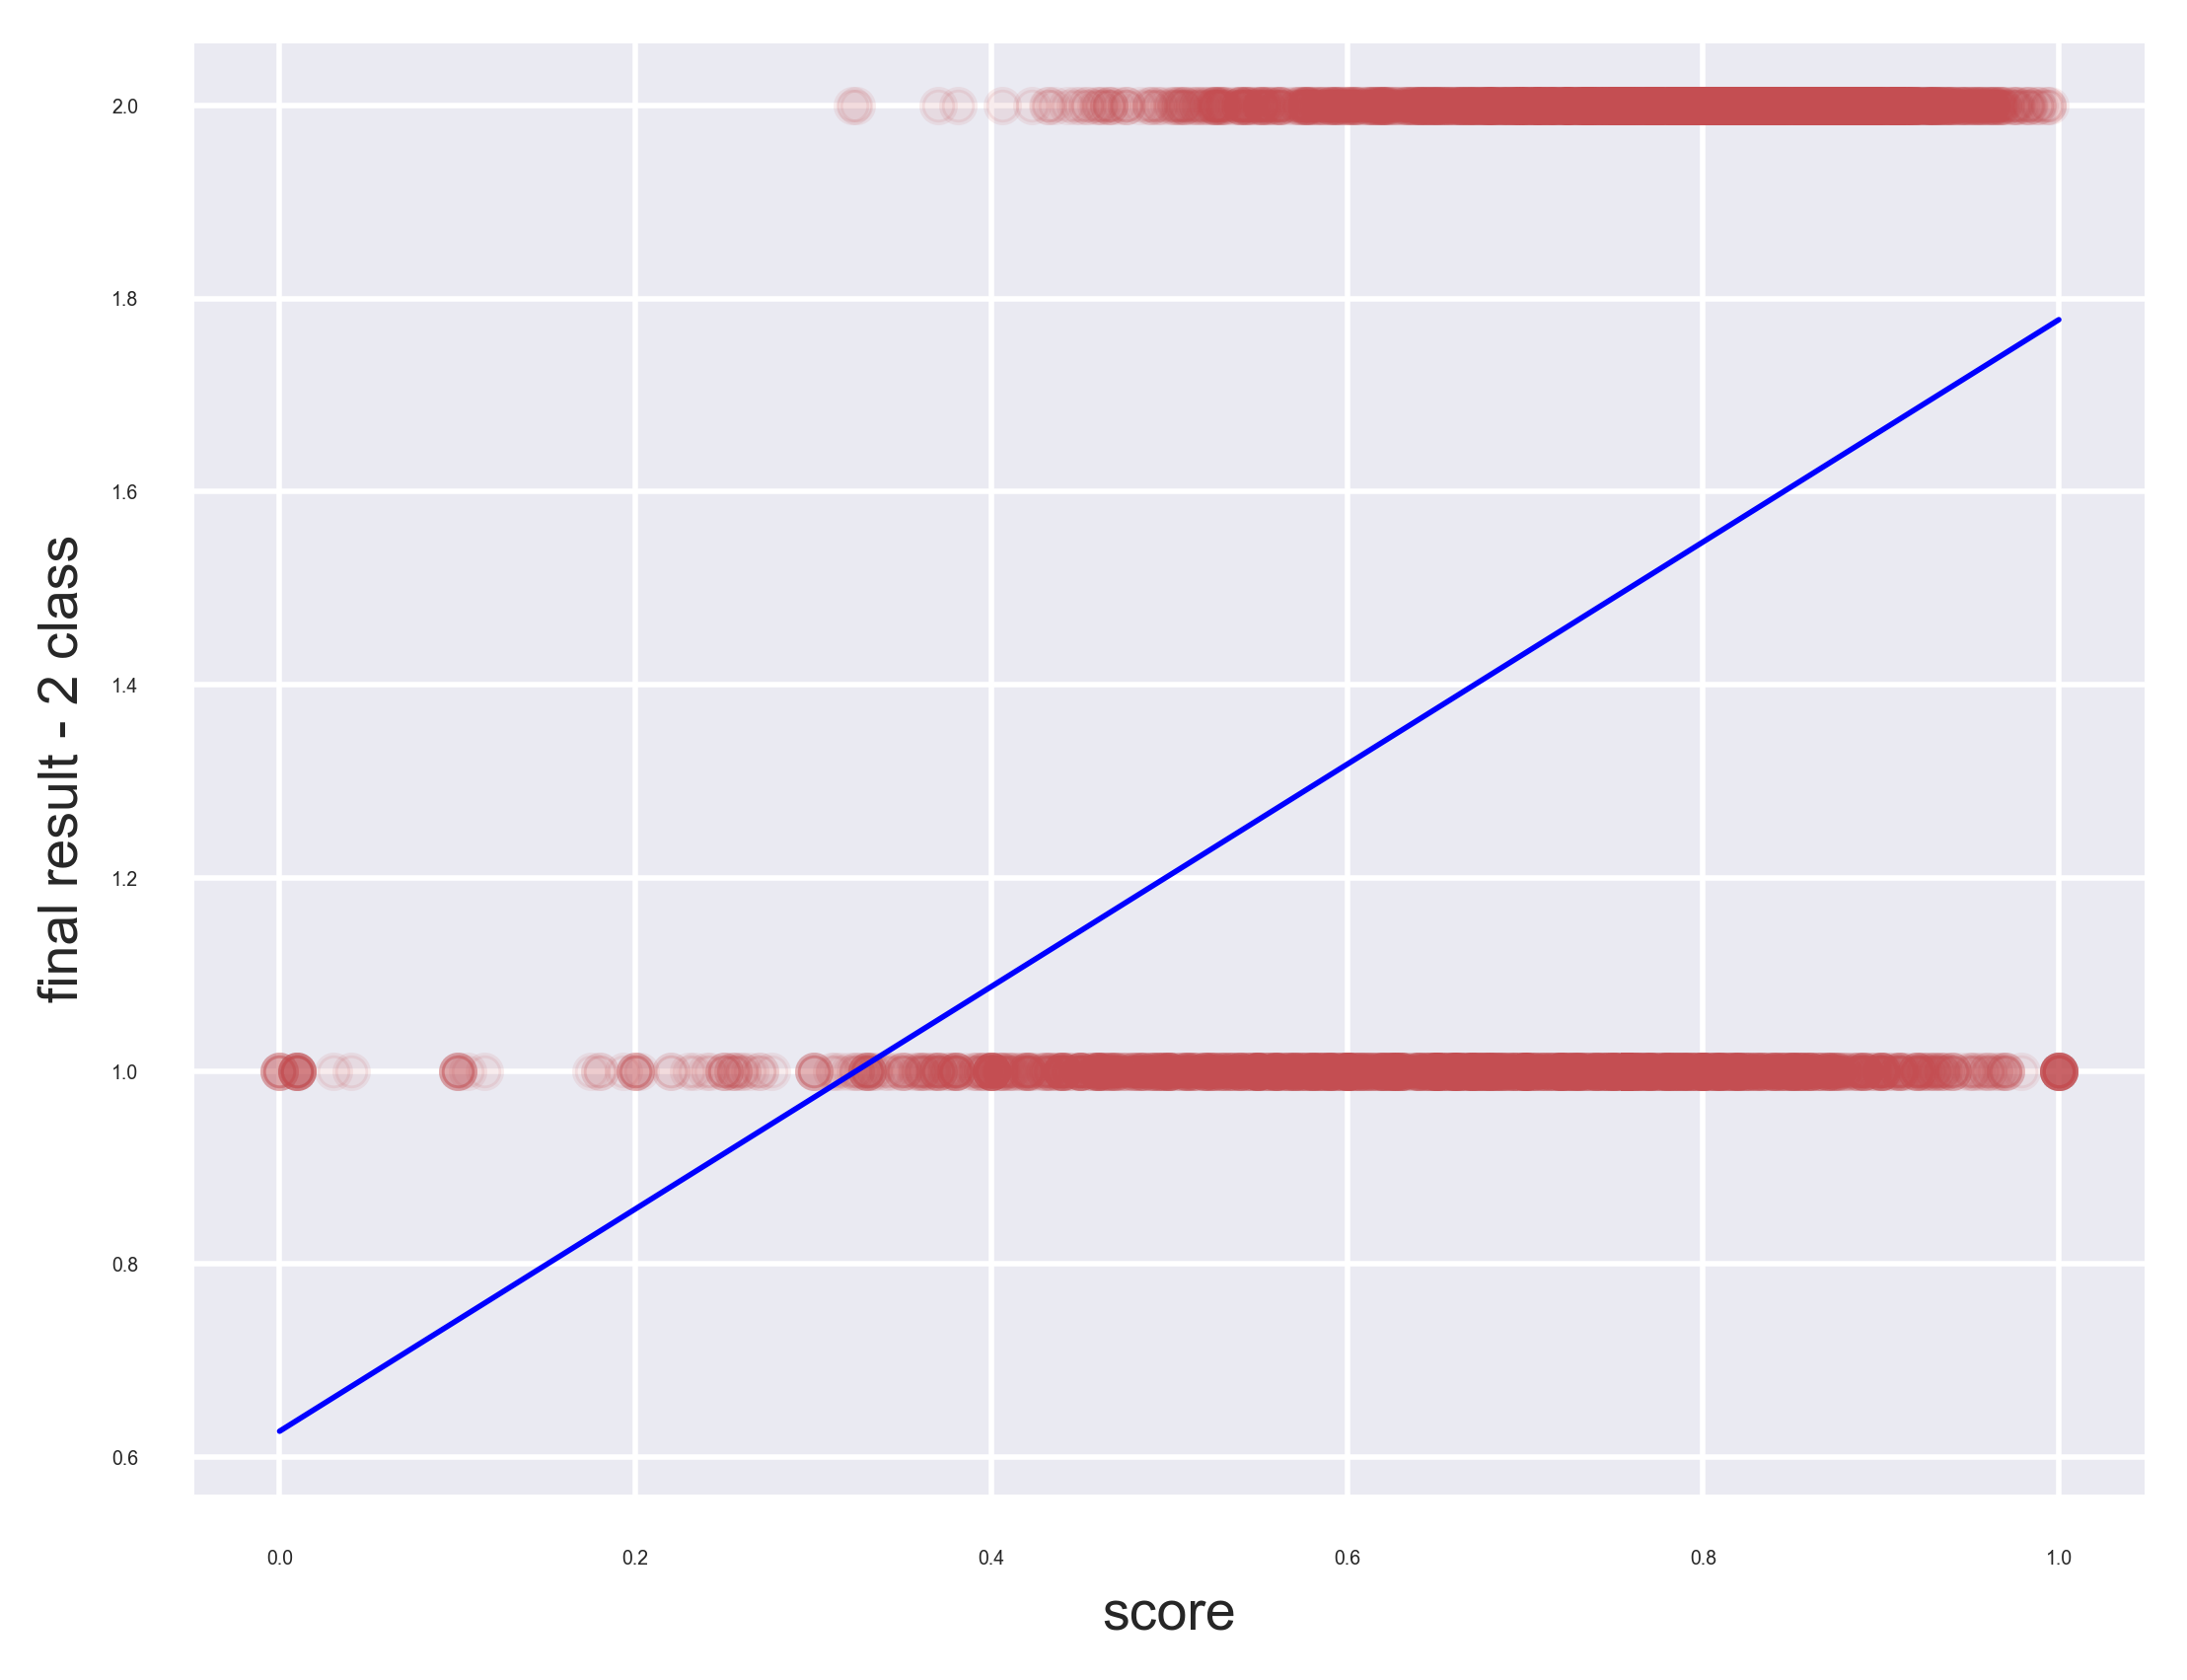
\includegraphics[width=\linewidth]{LinearRegression_2_class_model_against_score.png} 
	\caption{Linear Regression (2 class) against score}
	\label{fig:LinScore}
\end{figure}

\centering
\begin{figure}[H]
	\vspace{-0.4cm}
	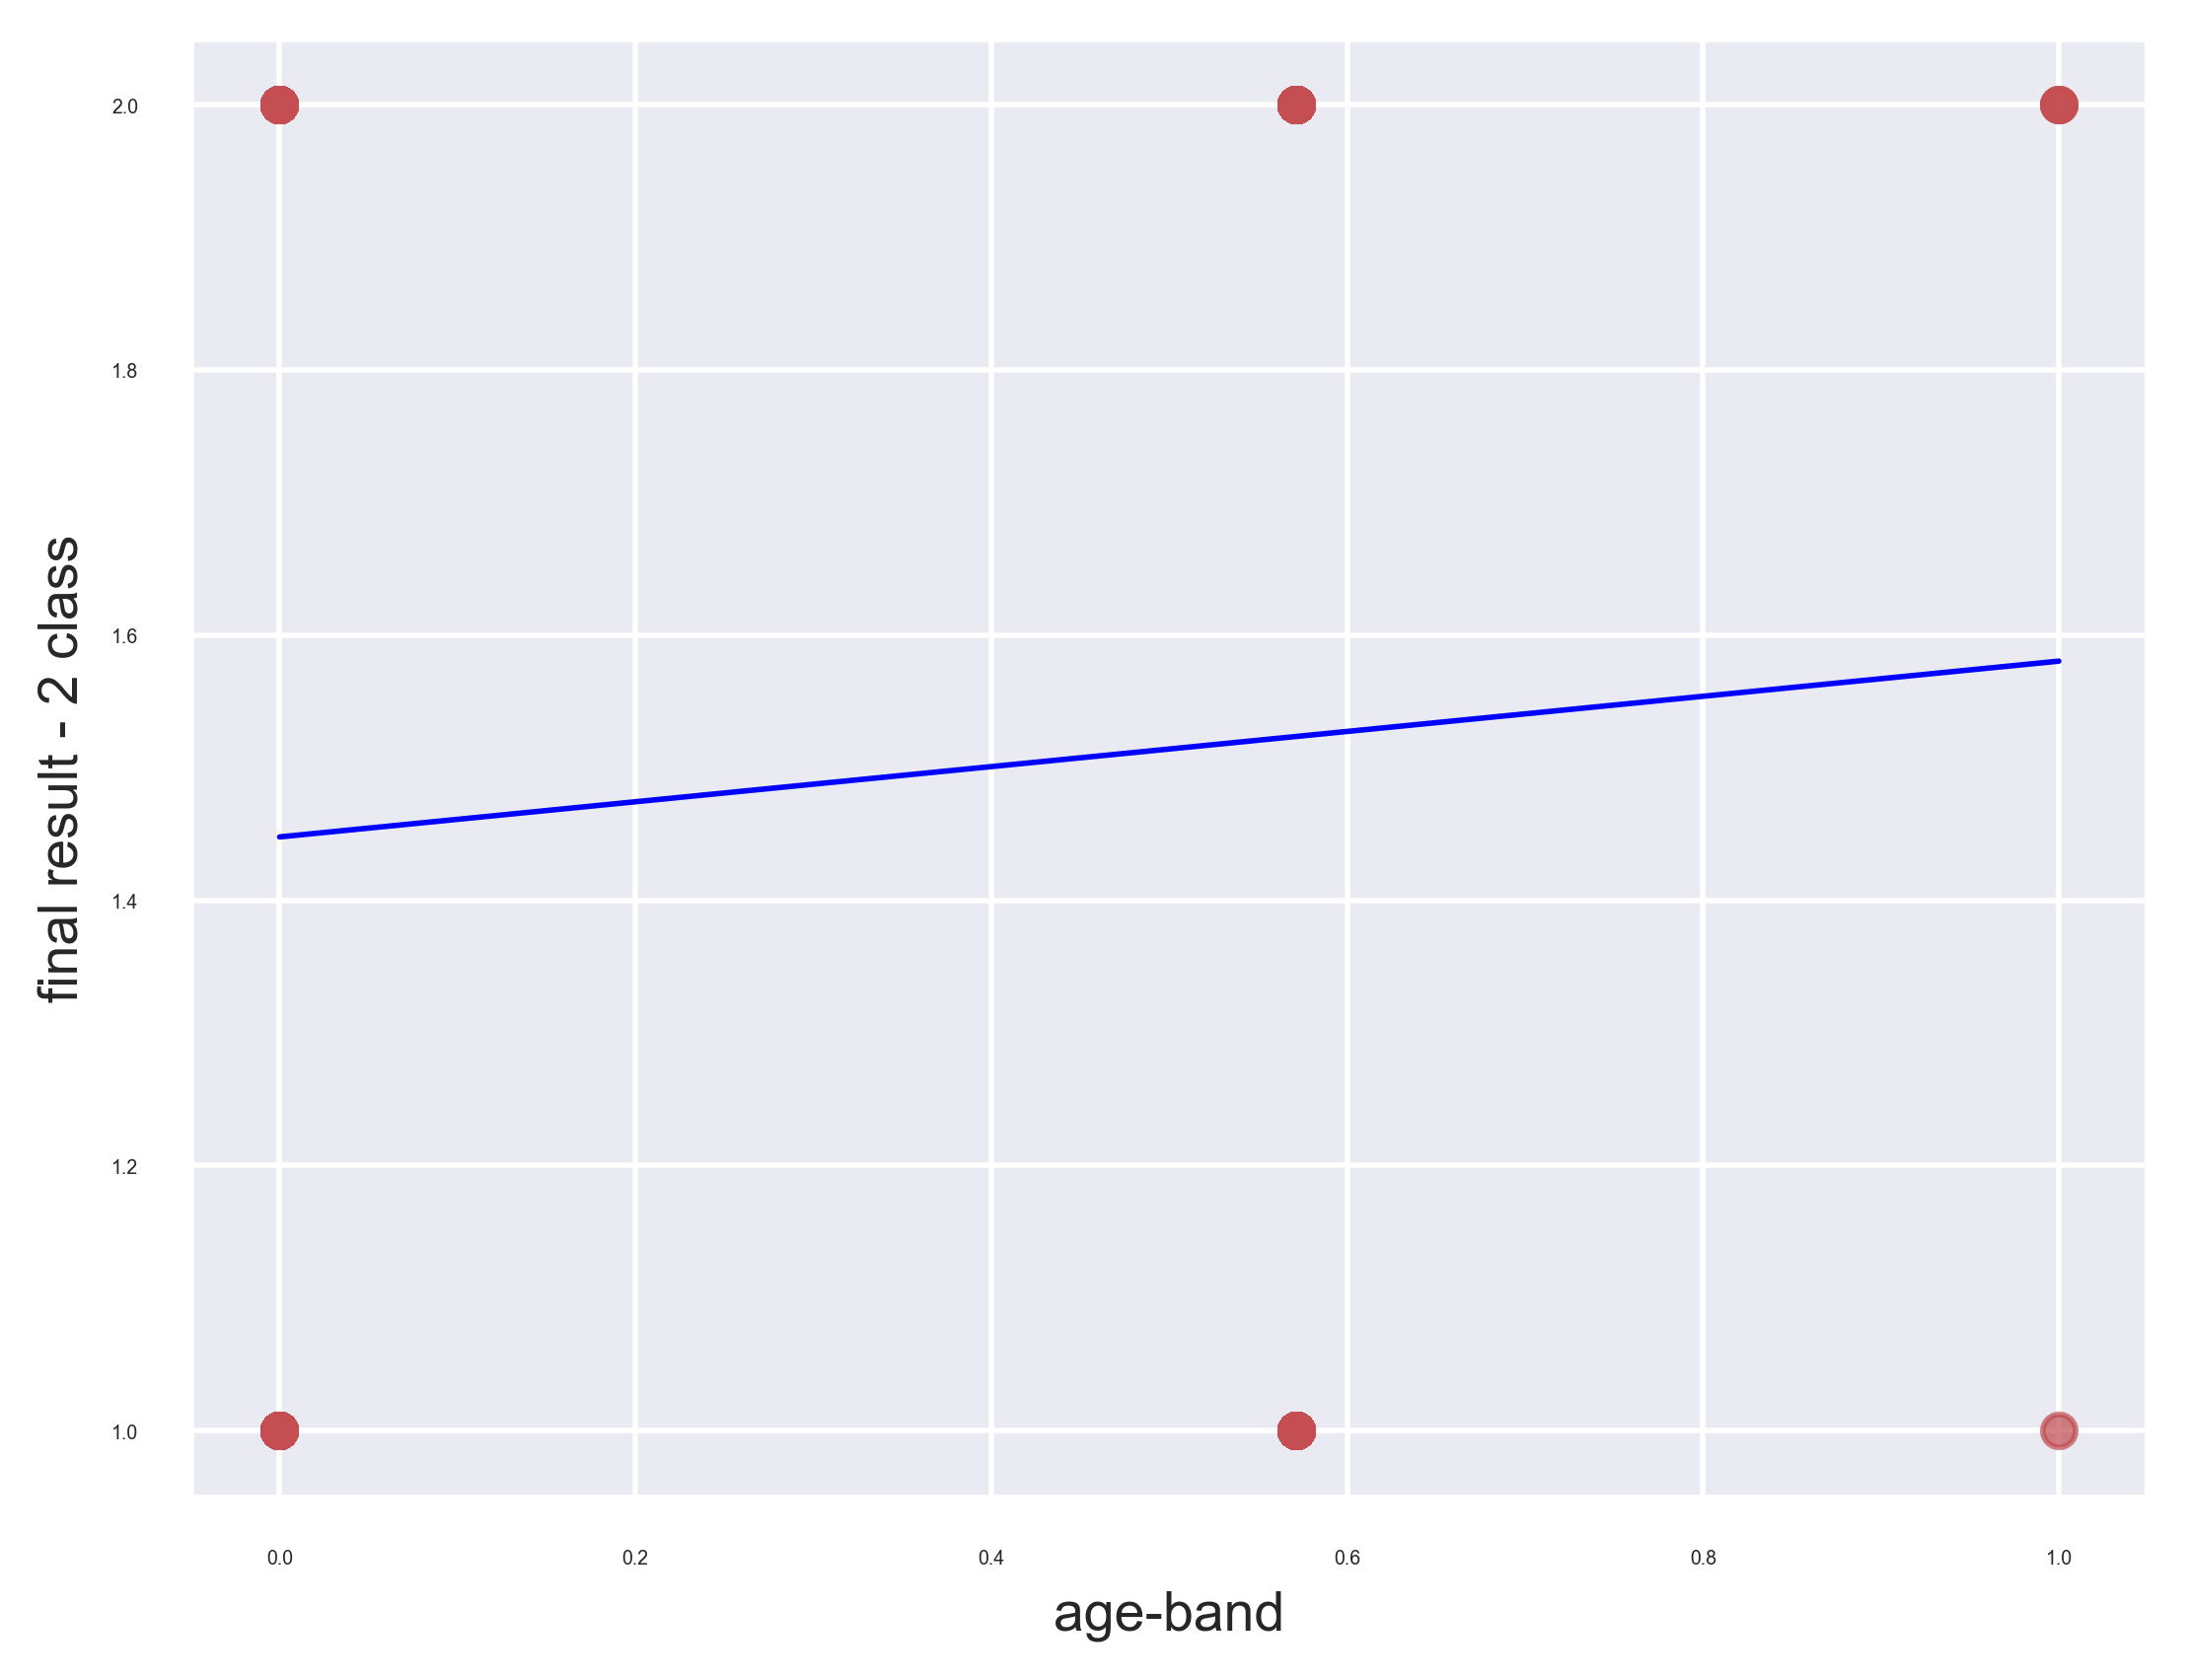
\includegraphics[width=\linewidth]{LinearRegression_2_class_model_against_age-band.png} 
	\caption{Linear Regression (2 class) against age-band}
	\label{fig:LinAge}
\end{figure}

\centering
\begin{figure}[H]
	\vspace{-0.4cm}
	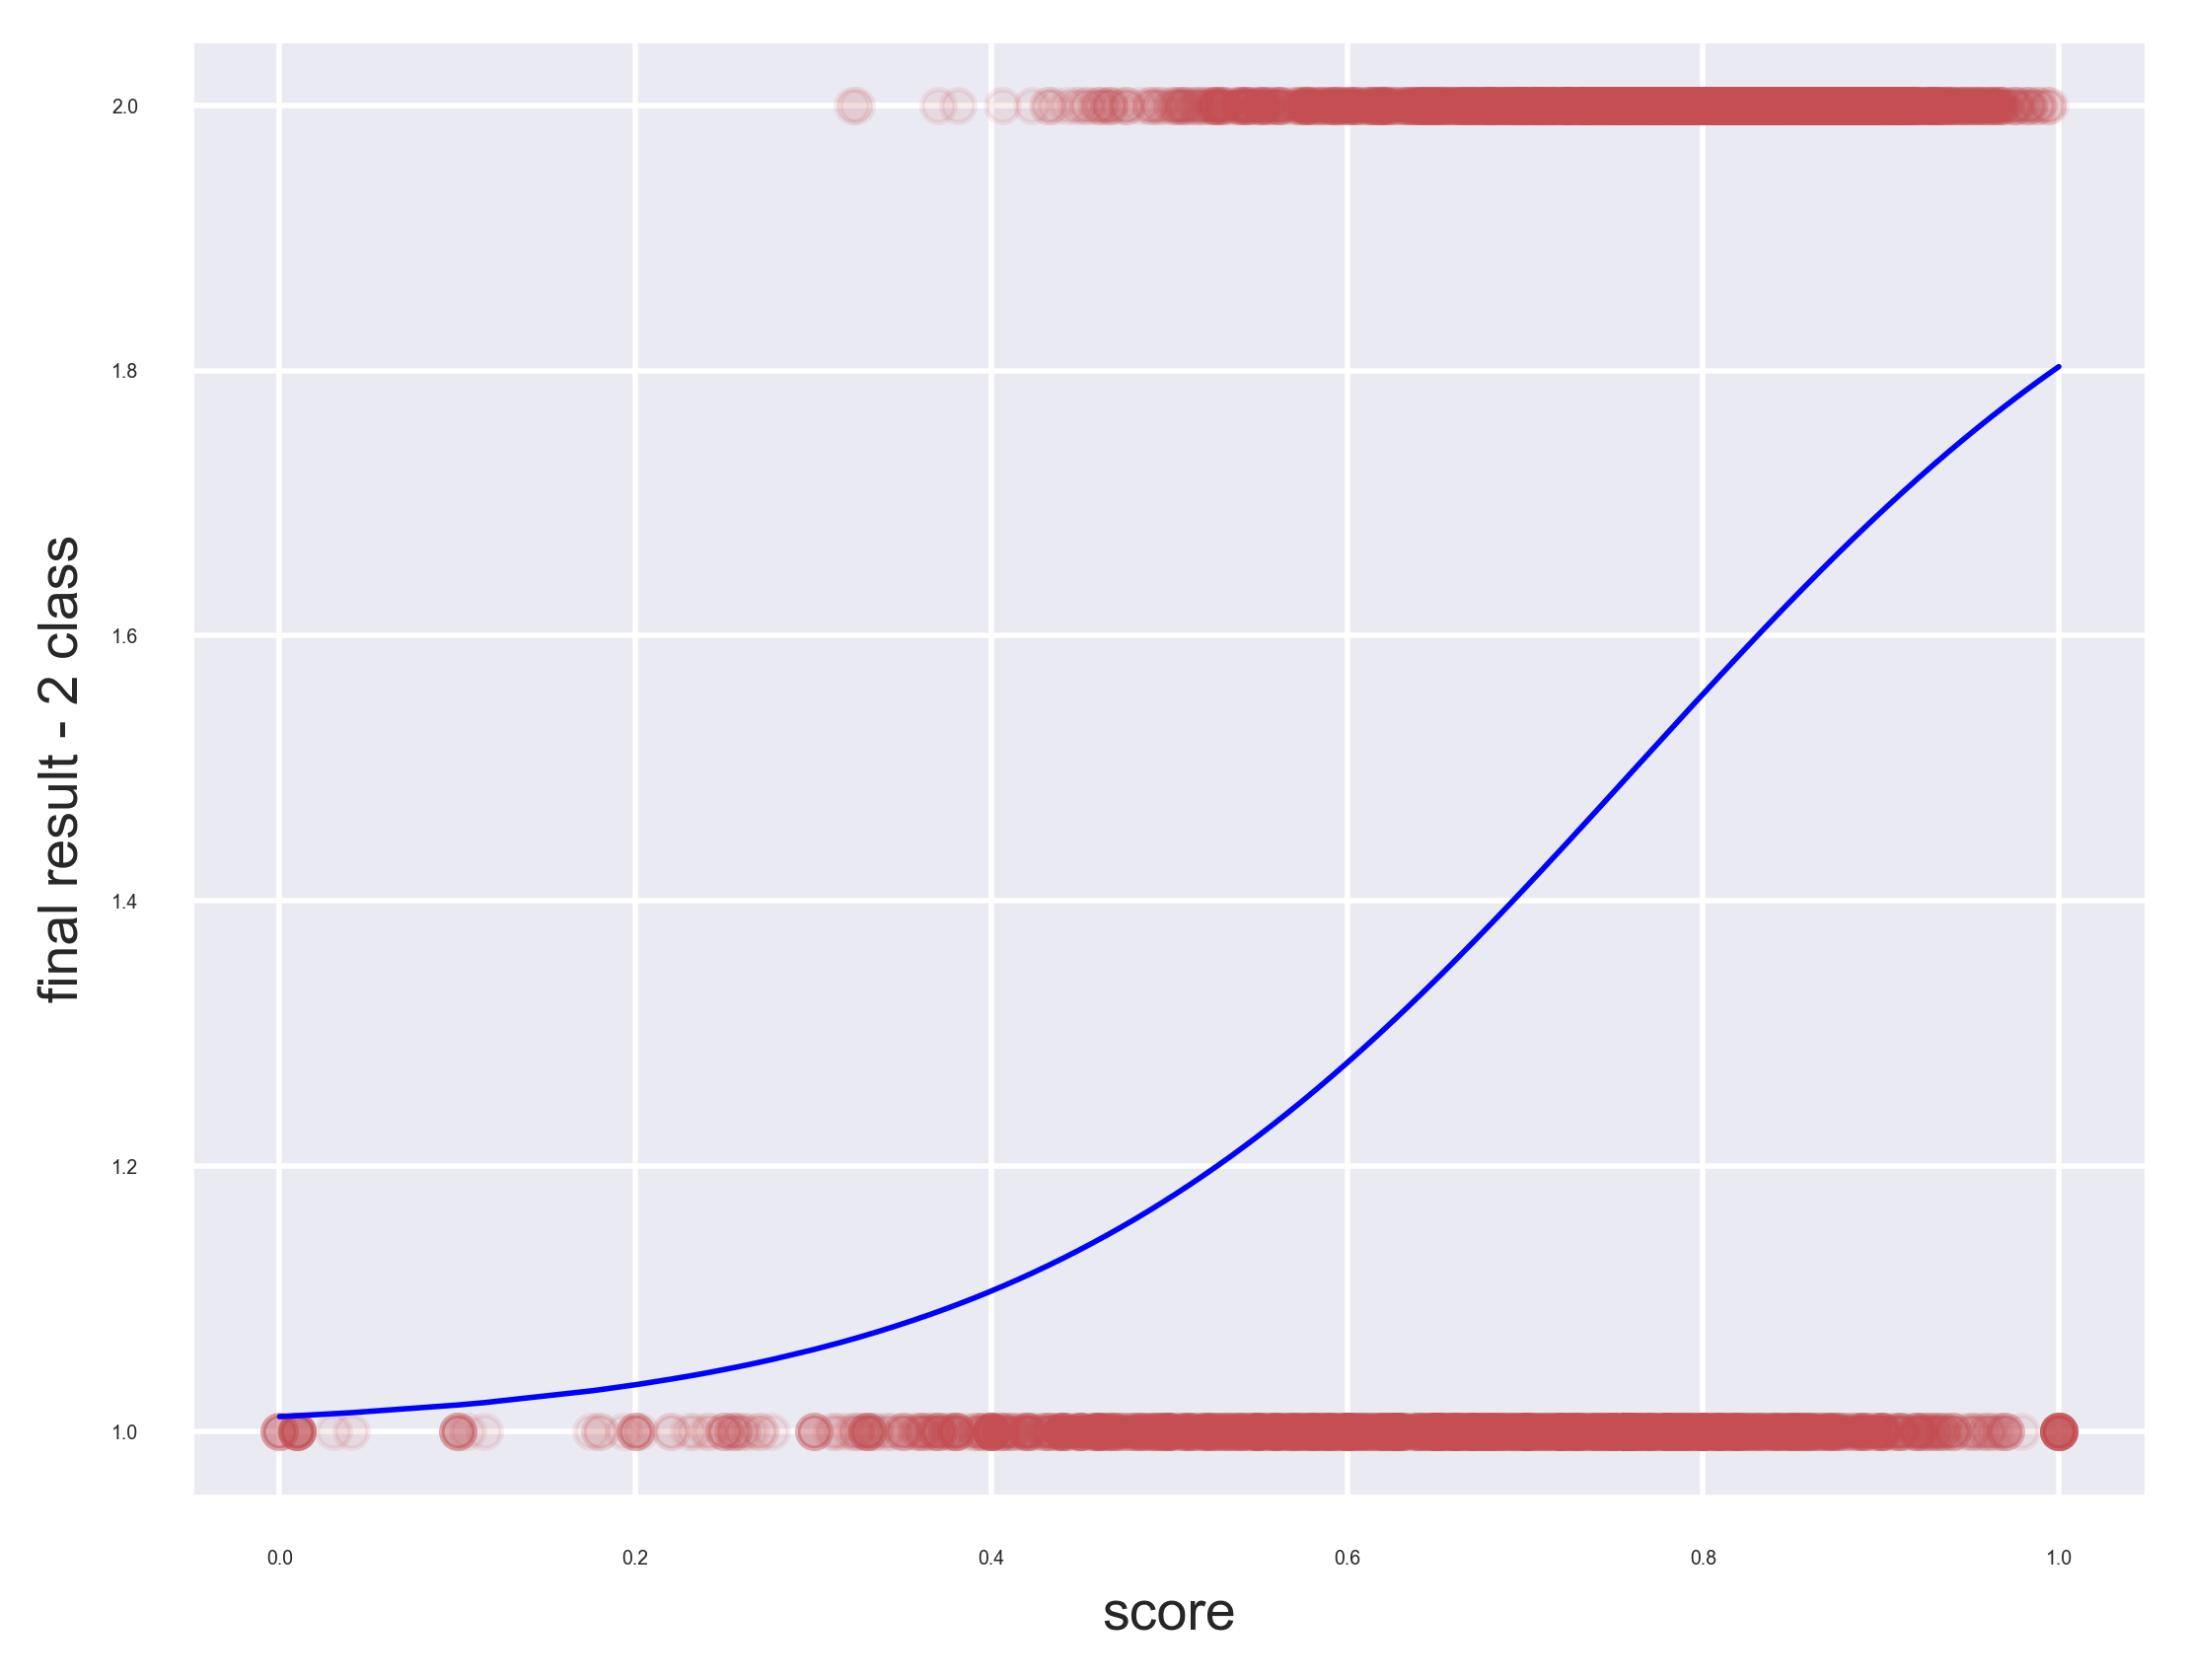
\includegraphics[width=\linewidth]{LogisticRegression_2_class_model_against_score.png} 
	\caption{Logistic Regression (2 class) against score}
	\label{fig:LogScore}
\end{figure}

\centering
\begin{figure}[H]
	\vspace{-0.4cm}
	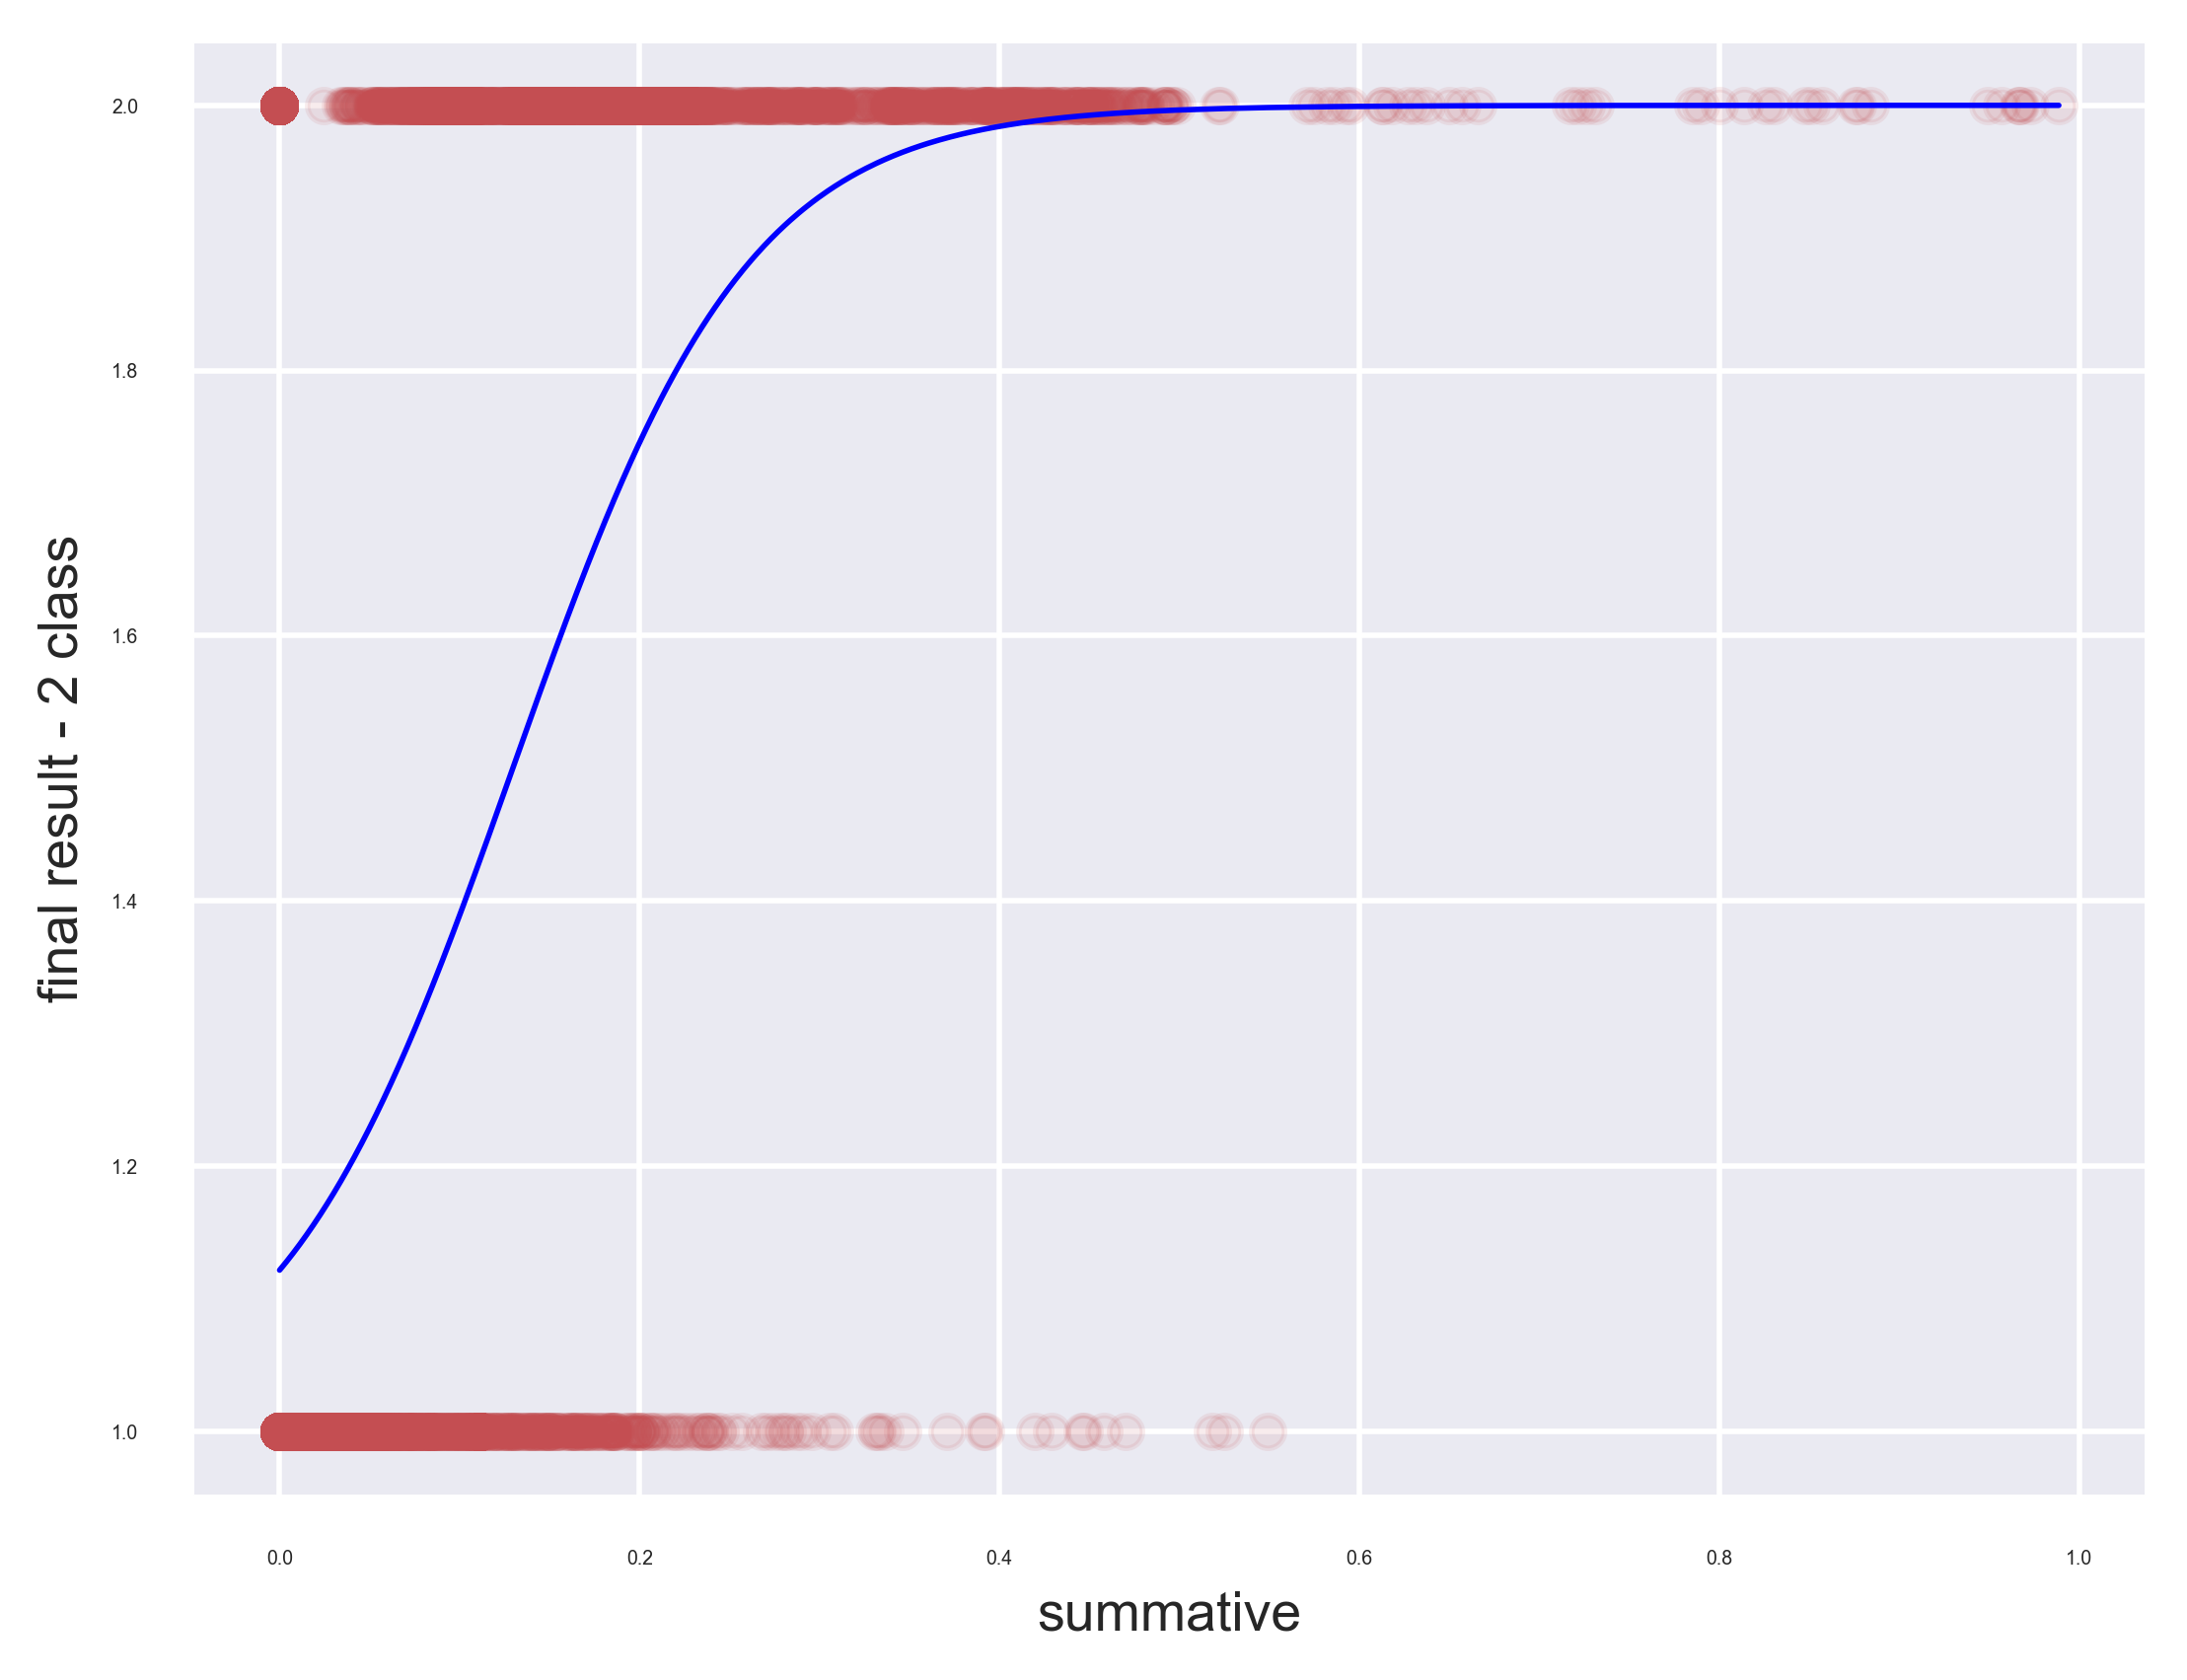
\includegraphics[width=\linewidth]{LogisticRegression_2_class_model_against_summative.png} 
	\caption{Logistic Regression (2 class) against summative}
	\label{fig:LogSumm}
\end{figure}

\centering
\begin{figure}[H]
	\vspace{-0.4cm}
	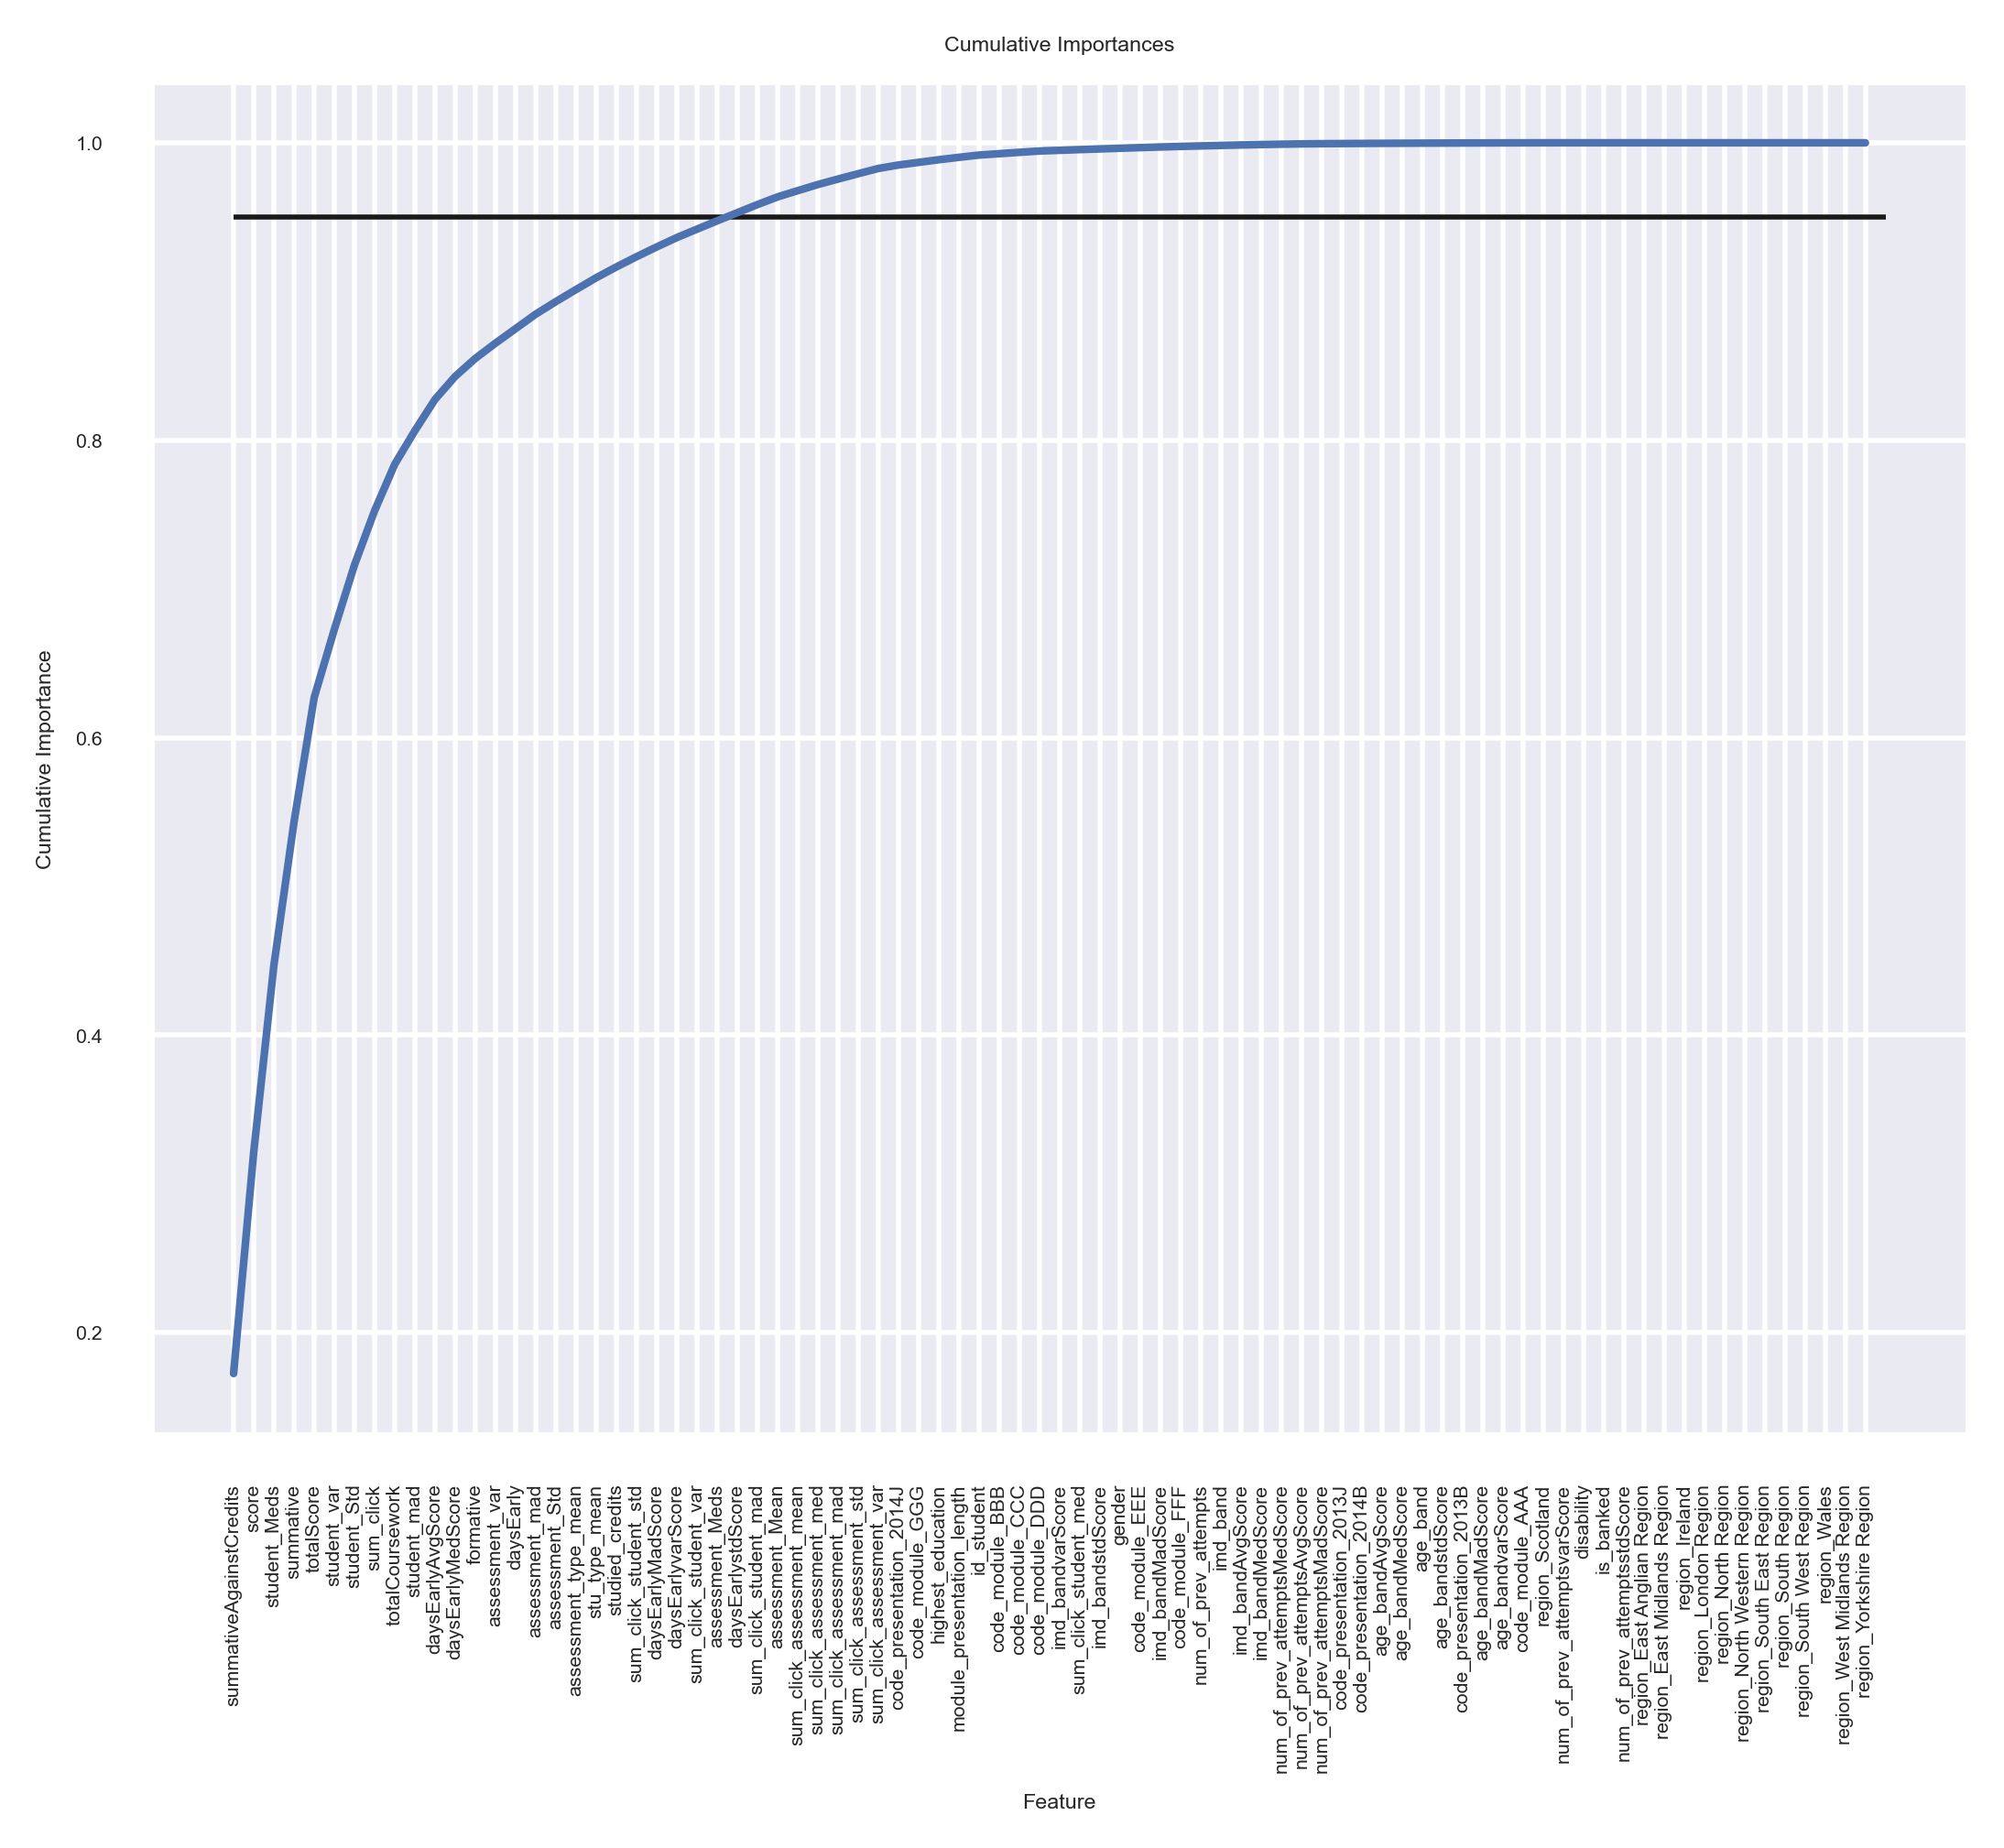
\includegraphics[width=\linewidth]{Importances.png}
	\caption{Cumulative Importances of Features}
	\label{fig:importances}
\end{figure}

\centering
\begin{figure}[H]
	\vspace{-0.4cm}
	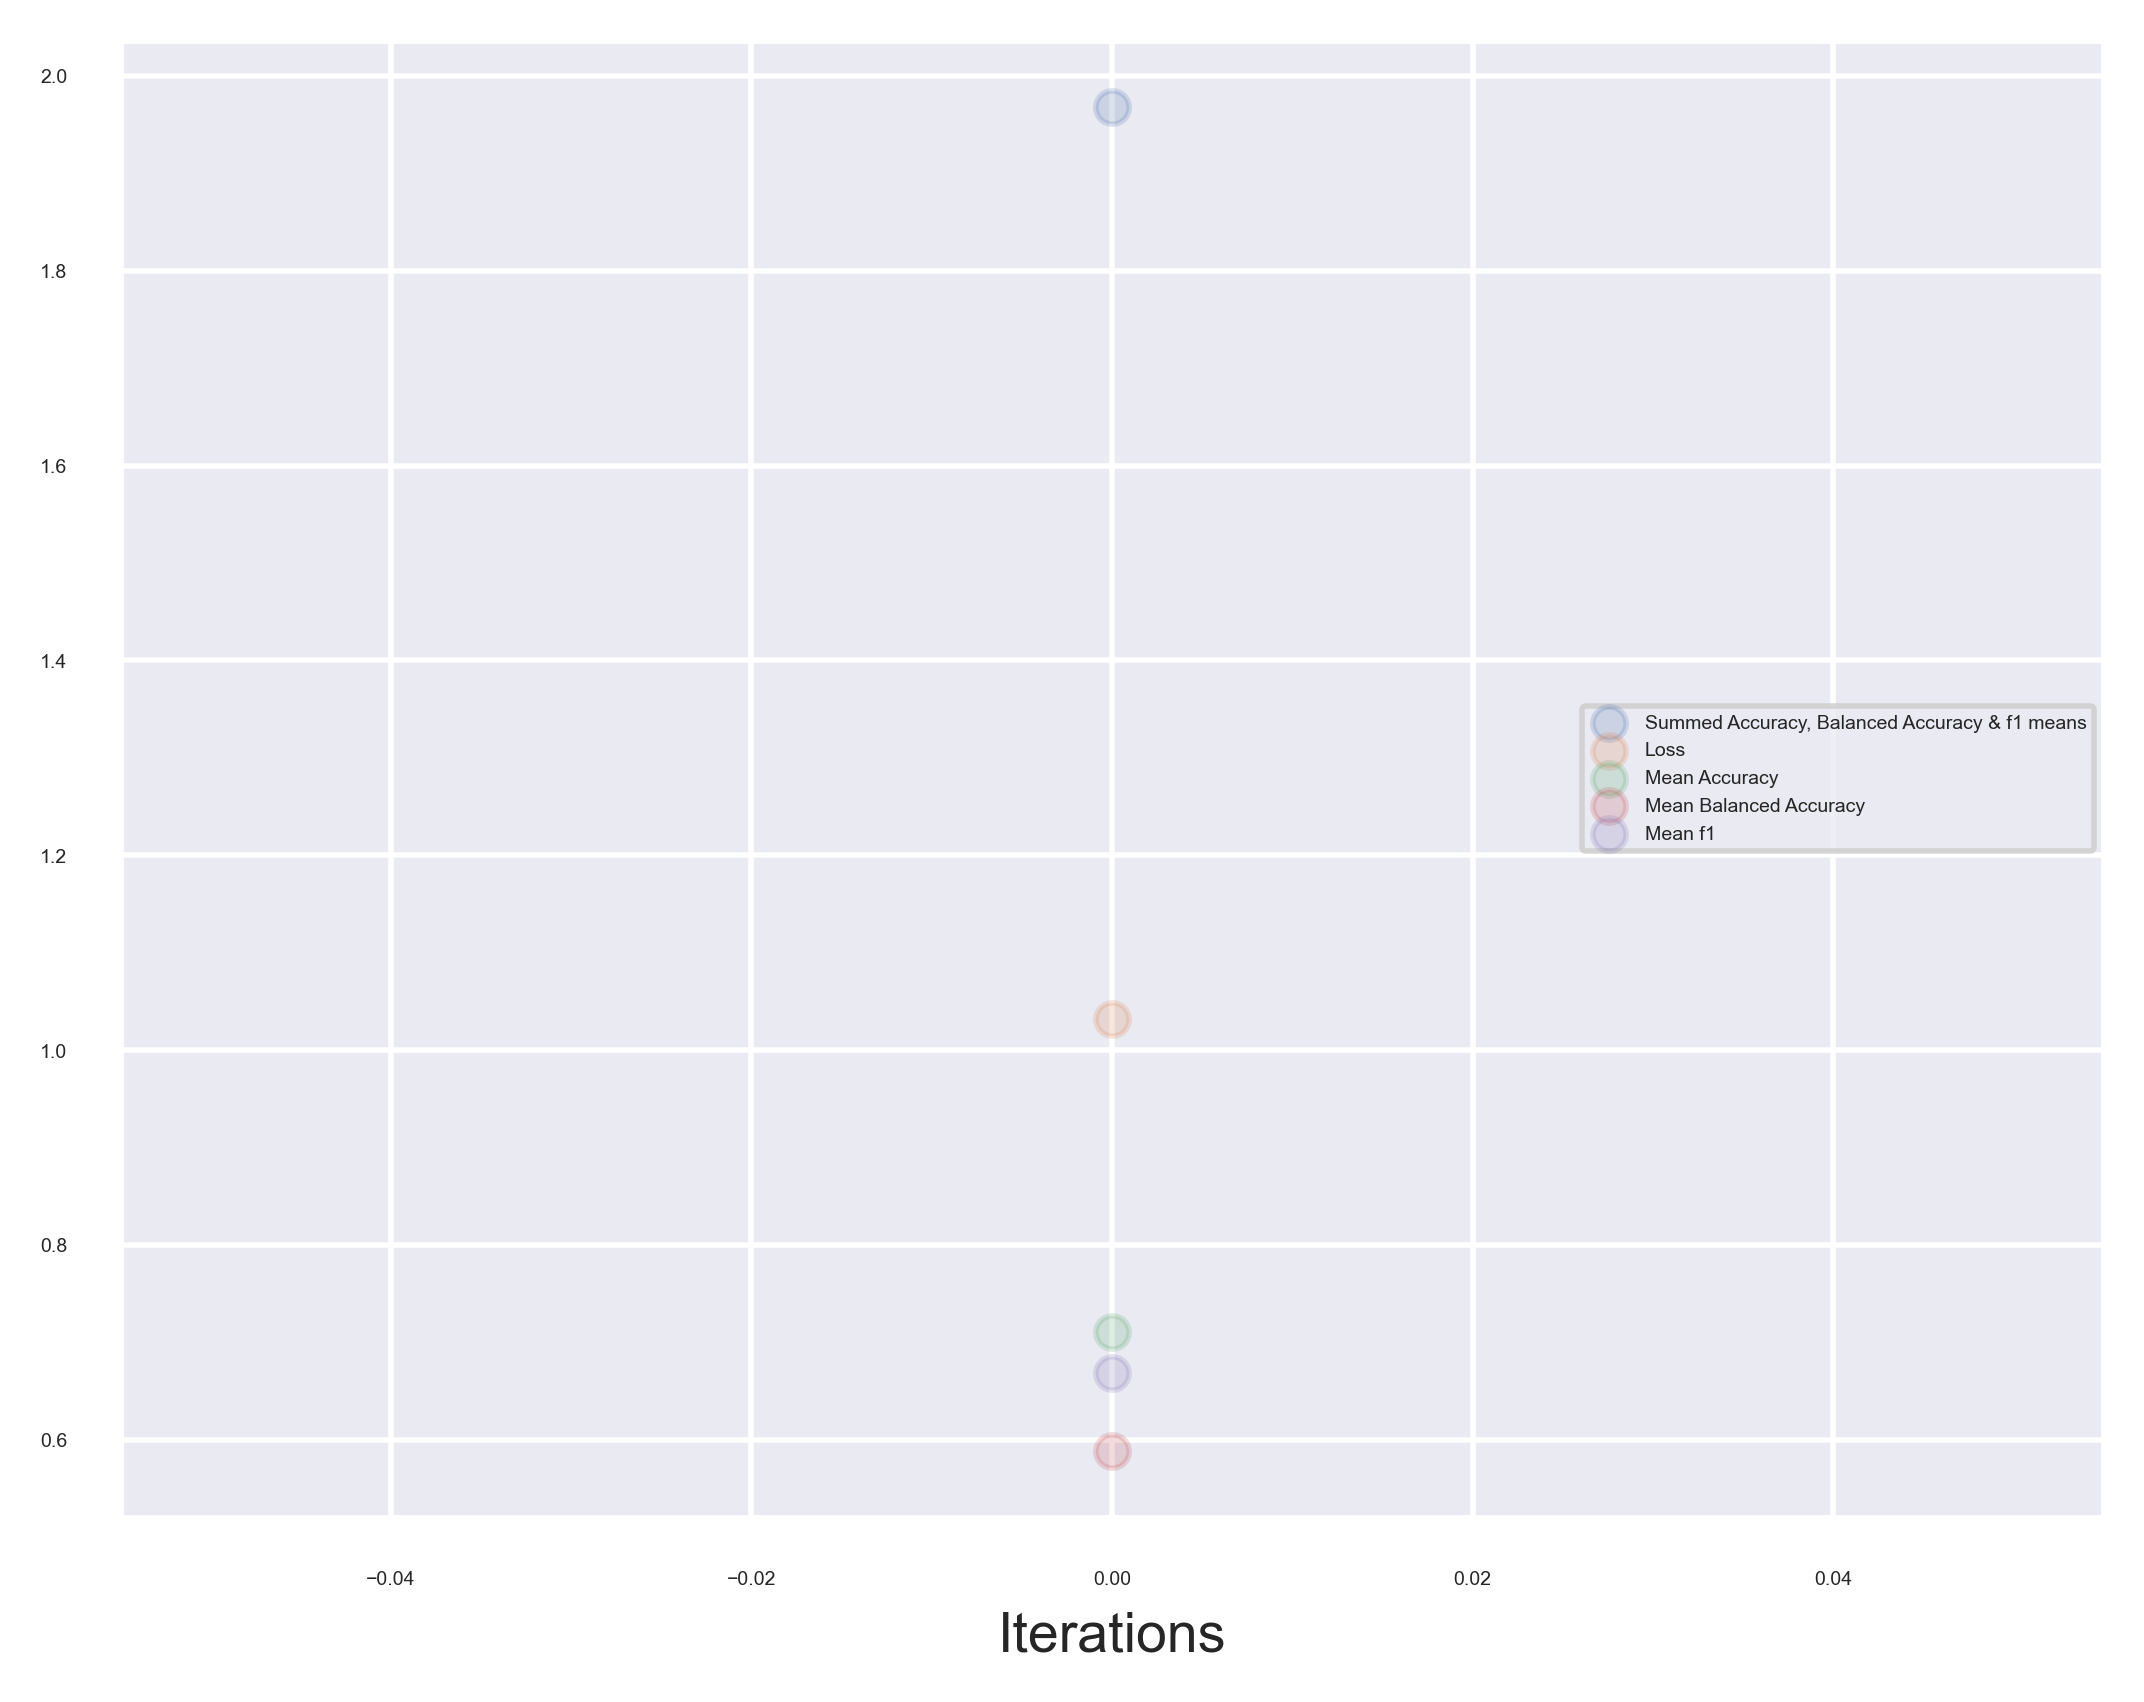
\includegraphics[width=\linewidth]{Accuracy_against_iteration1.png} 
	\caption{Metrics against iteration 1}
	\label{fig:Acc1}
\end{figure}

\centering
\begin{figure}[H]
	\vspace{-0.4cm}
	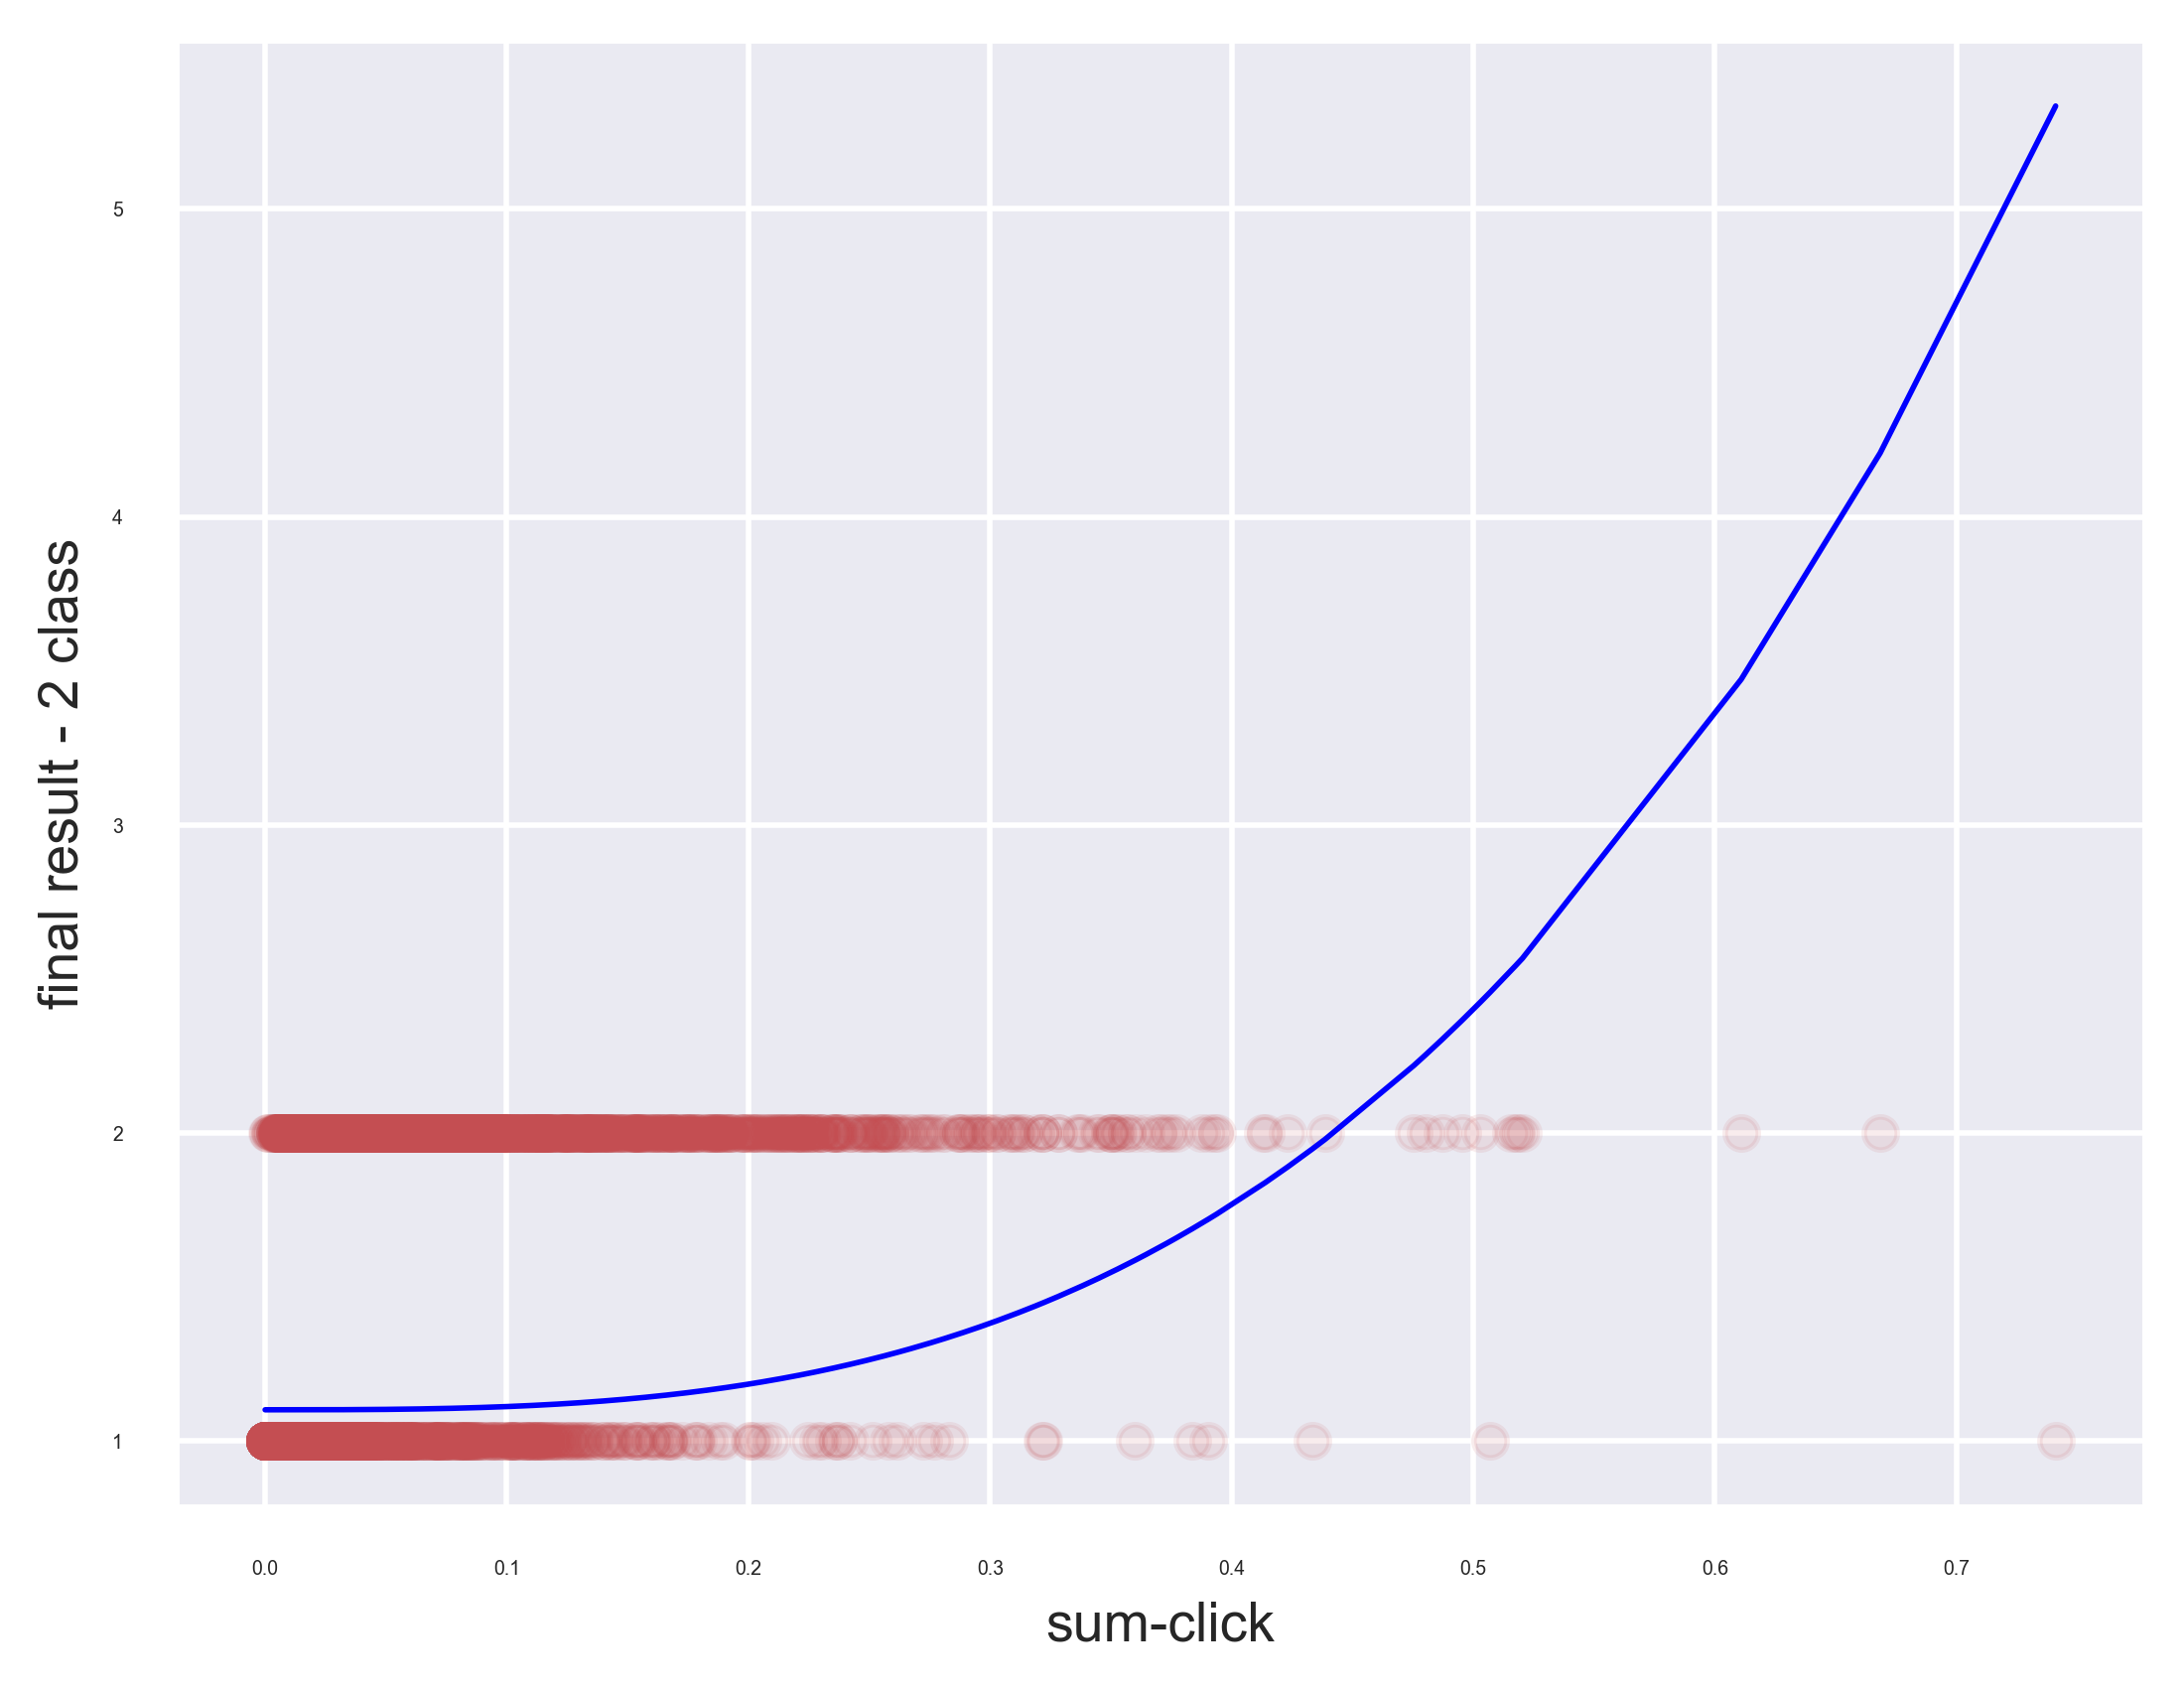
\includegraphics[width=\linewidth]{SVR-Polynomial-Kernel_2_class_model_against_sum-click.png} 
	\caption{SVR-Poly-Kernel (2 class) against sum-click}
	\label{fig:PolyClicks}
\end{figure}

\centering
\begin{figure}[H]
	\vspace{-0.4cm}
	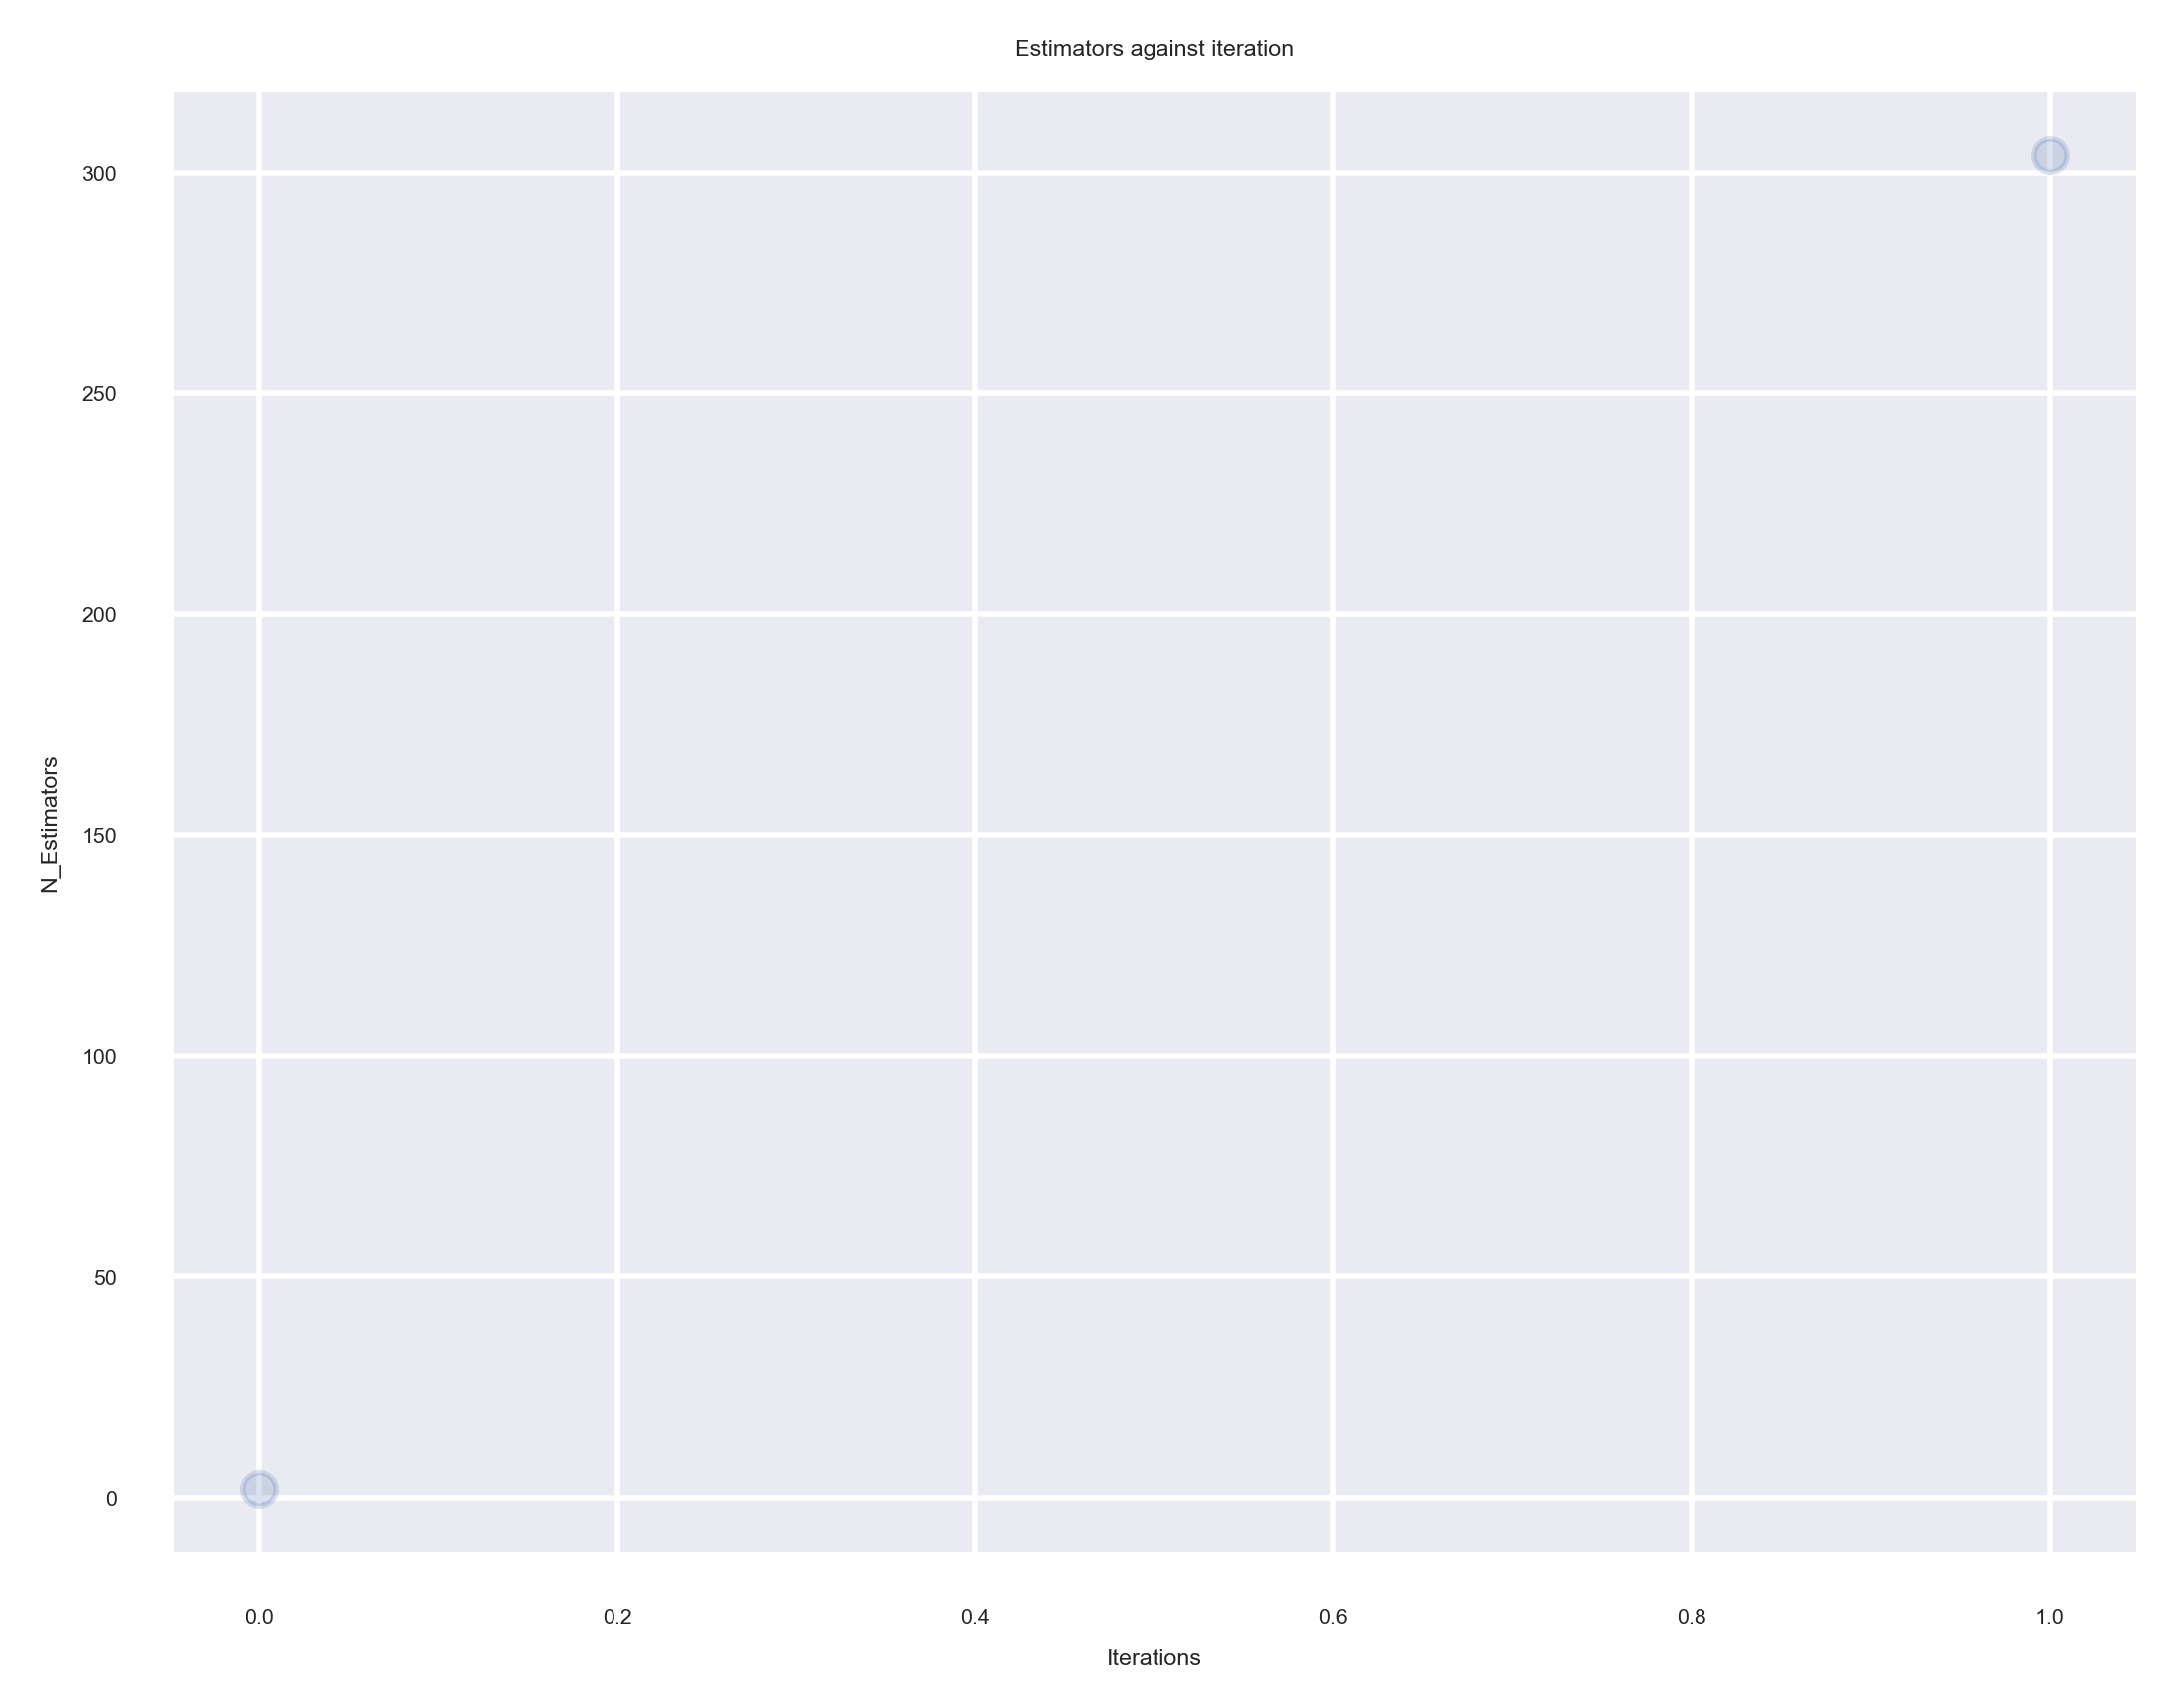
\includegraphics[width=\linewidth]{Estimators_against_iteration.png} 
	\caption{Selected n-Estimators againts iteration}
	\label{fig:estimators}
\end{figure}

\centering
\begin{figure}[H]
	\vspace{-0.4cm}
	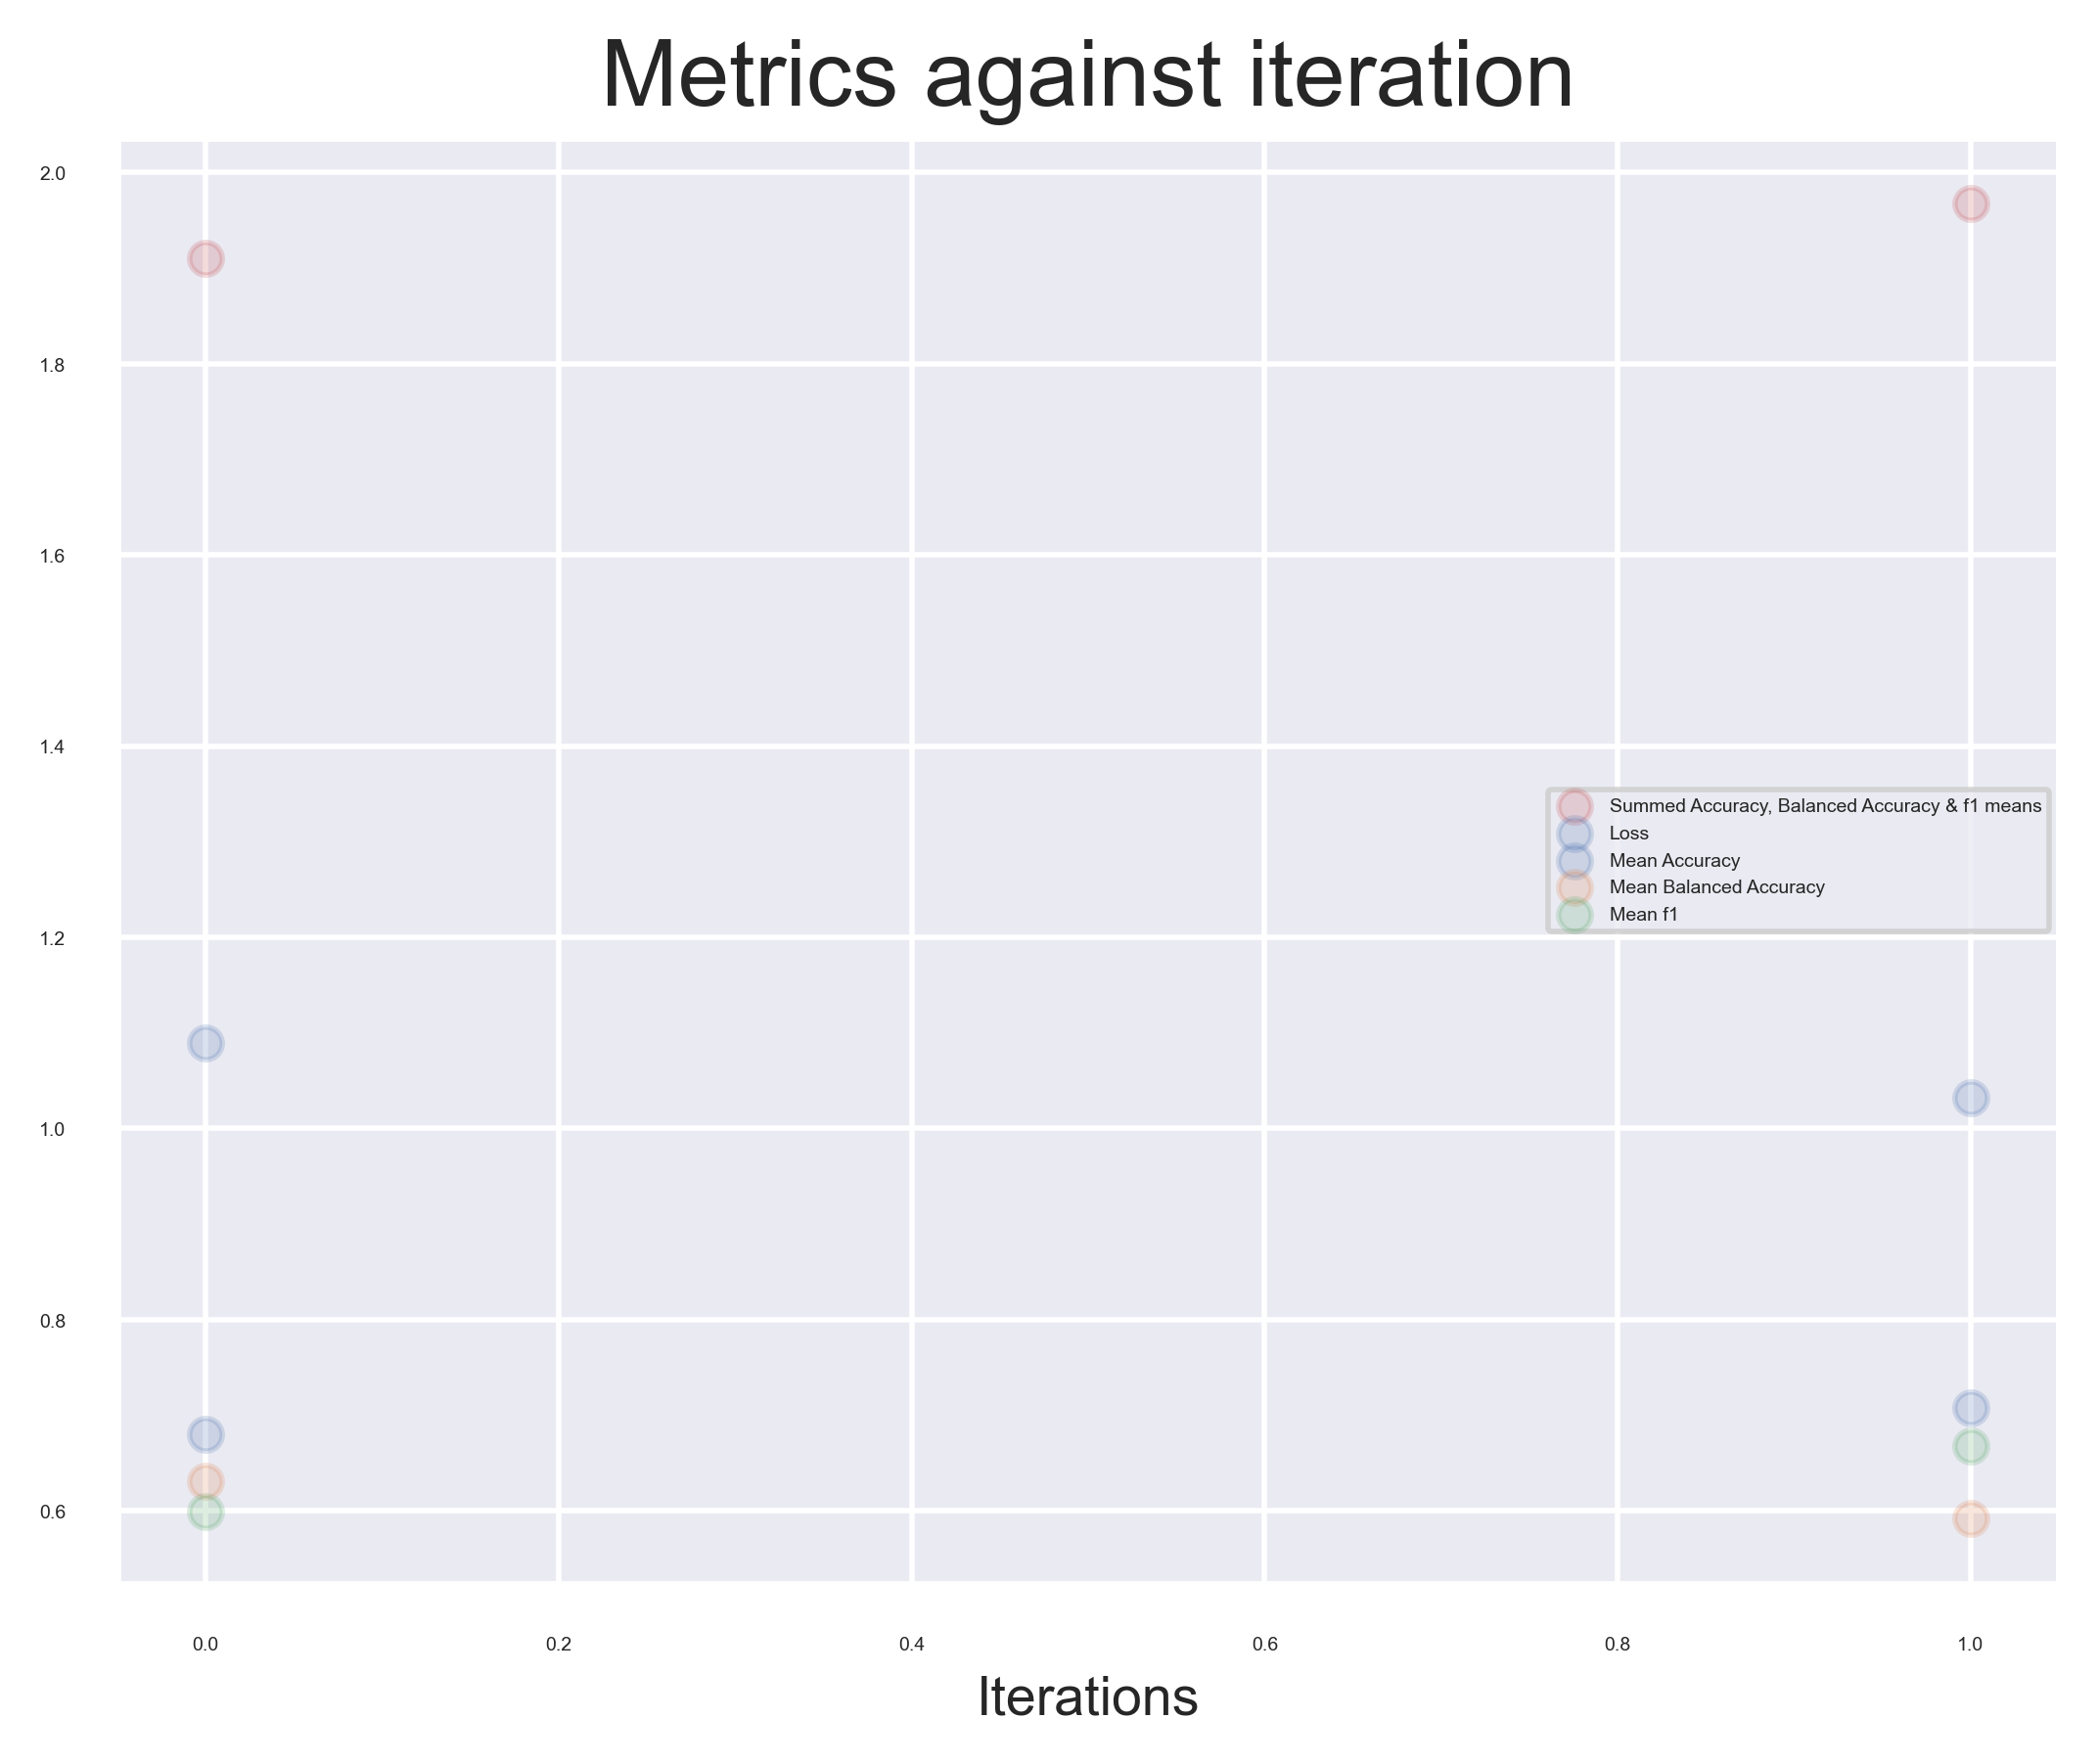
\includegraphics[width=\linewidth]{Accuracy_against_iteration2.png} 
	\caption{Metrics against iteration 2}
	\label{fig:Acc2}
\end{figure}

\end{multicols}
\begin{multicols}{3}
	\begin{table}[H]
		\centering
		\captionsetup{justification=centering,margin=1cm}
		\begin{tabular}{|l|l|l|l|}
			\hline
			Model                 & Class & Mean &SD \\ \hline
			Linear& 4 & 0.604 & 0.010 \\ \hline
			Logistic& 4 & 0.702 & 0.007 \\ \hline
			- & 3 & 0.767 & 0.005 \\ \hline
			- & 2 & 0.915 & 0.003 \\ \hline
			SVR Linear & 4 & 0.575 & 0.013 \\ \hline
			SVR Poly & 4 & 0.746 & 0.008 \\ \hline
			SVR RBF & 4 & 0.723 & 0.009 \\ \hline
			SVC & 4 & 0.681 & 0.007 \\ \hline
			- & 3 & 0.782 & 0.005 \\ \hline
			- & 2 & 0.932 & 0.003 \\ \hline
			DT& 4 & 0.674 & 0.003 \\ \hline
			- & 3 & 0.755 & 0.005 \\ \hline
			- & 2 & 0.915 & 0.002 \\ \hline
			RF & 4 & 0.748 & 0.005 \\ \hline
			- & 3 & 0.809 & 0.005 \\ \hline
			- & 2 & 0.942 & 0.003 \\ \hline
			\end{tabular}
		\caption{Model Selection CV Accuracy Metrics}
		\label{table:modelSelection}
	\end{table}

	\begin{table}[H]
		\centering
		\captionsetup{justification=centering,margin=1cm}
		\begin{tabular}{|l|l|l|l|l|}
			\hline
							&	With 	&  Fail & Pass  & Dist \\ \hline
			With      &  	2056 		&  462  &   22  &         4 \\ \hline
			Fail           &   606 		&  841  & 251   &         3 \\ \hline
			Pass          &     8  		&  205  & 2615  &        293 \\ \hline
			Dist     &     0  		&   0   & 248   &       535 \\ \hline
			\end{tabular}
		\centering
		\caption{RF 4 Class \\Confusion Matrix}
		\label{table:RF4Confusion}
	\end{table}


	\begin{table}[H]
		\centering
		\captionsetup{justification=centering,margin=1cm}
		\begin{tabular}{|l|l|l|}
			\hline
				 &	Fail  & Pass \\ \hline
			Fail &  3937  & 308  \\ \hline
			Pass &    60  & 3844 \\ \hline
			\end{tabular}
		\centering
		\caption{RF 2 Class \\Confusion Matrix}
		\label{table:RF2Confusion}
	\end{table}

	\begin{table}[H]
		\centering
		\captionsetup{justification=centering,margin=1cm}
		\begin{tabular}{|l|l|l|l|l|}
			\hline
							&	With 	&  Fail & Pass  & Dist \\ \hline
			With      &  	2097 		&  373  &   72  &         2 \\ \hline
			Fail           &   723 		&  640  &  335  &         3 \\ \hline
			Pass        &     84  		&  125  & 2748  &        164 \\ \hline
			Dist     &     1 		&   3   & 390  &       389 \\ \hline
			\end{tabular}
		\centering
		\caption{Logistic 4 Class \\Confusion Matrix}
		\label{table:Log4Confusion}
	\end{table}

	\vspace{2.2cm}

	\begin{table}[H]
		\centering
		\captionsetup{justification=centering,margin=1cm}
		\begin{tabular}{|l|l|l|}
			\hline
				 &	Fail  & Pass \\ \hline
			Fail &  3889  & 356  \\ \hline
			Pass &   261  & 3643 \\ \hline
			\end{tabular}
		\centering
		\caption{Logistic 2 Class \\Confusion Matrix}
		\label{table:Log2Confusion}
	\end{table}
\end{multicols}

		

	

\begin{figure}[H]
	\centering
	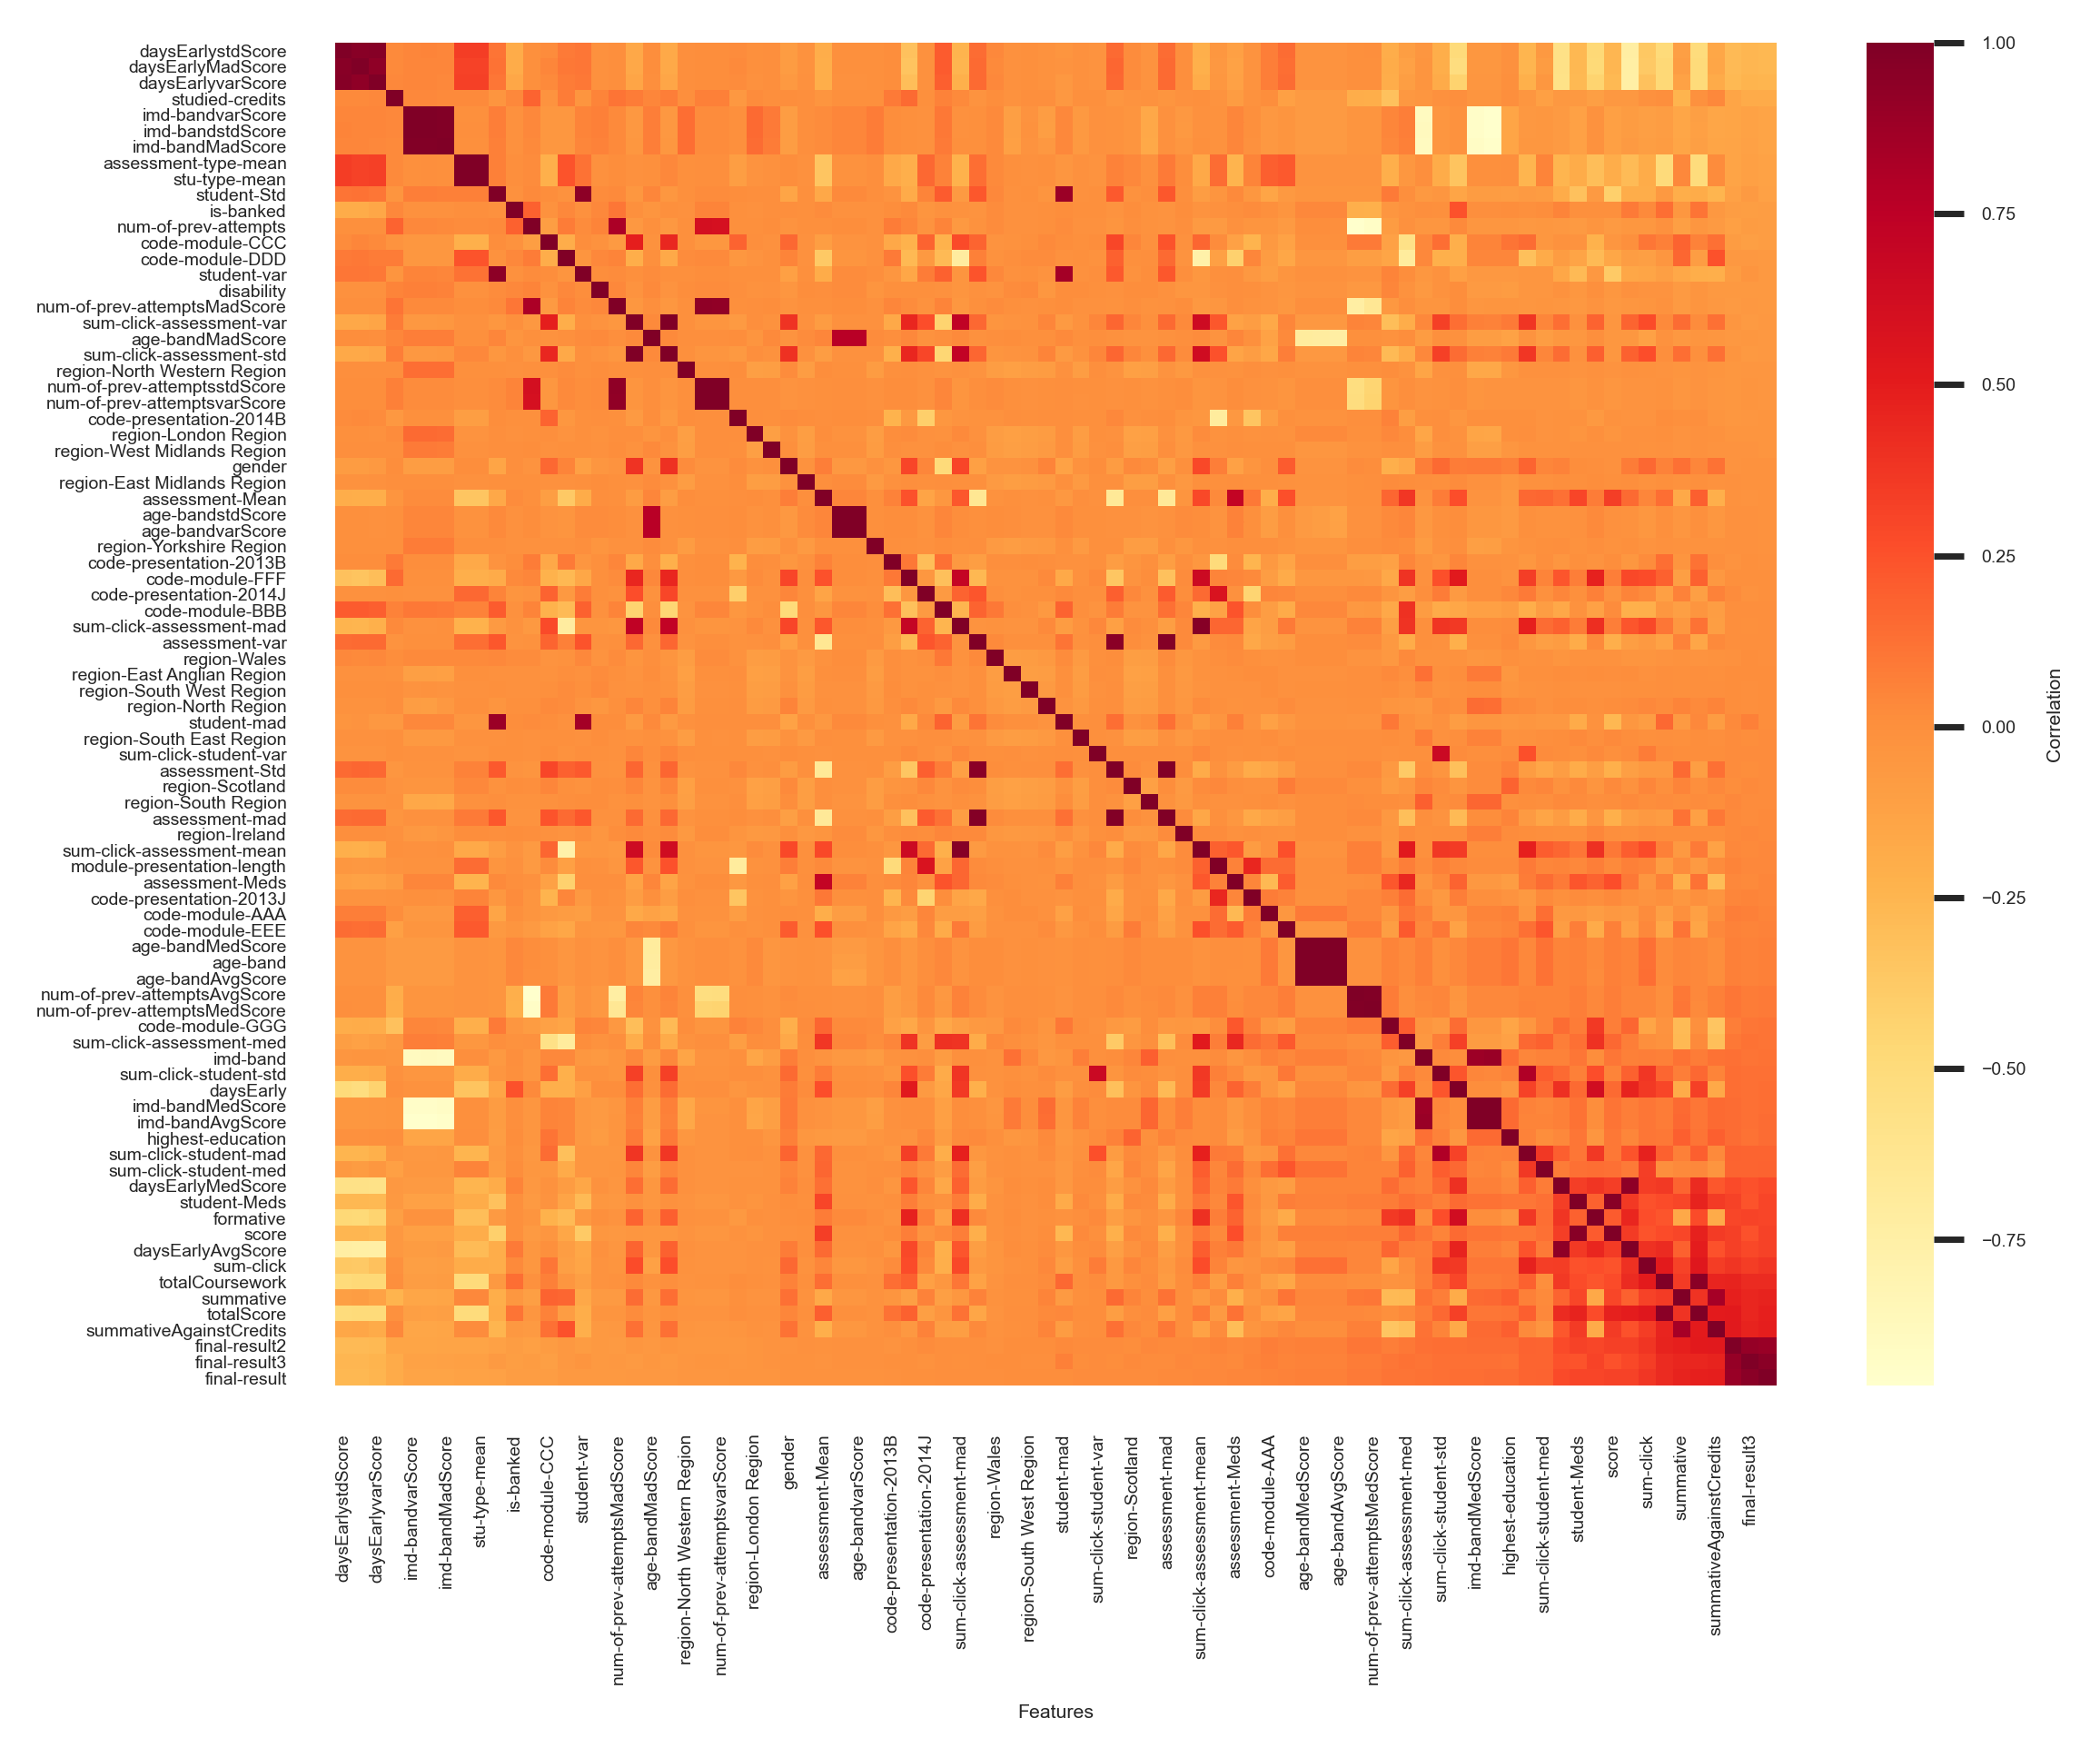
\includegraphics[width=0.95\linewidth]{heatmap.png} 
	\caption{Correlation Heatmap}
	\label{fig:heatmap}
\end{figure}

\end{document}
